\documentclass{article}
\usepackage[utf8]{inputenc}
\usepackage[T1]{fontenc}
\usepackage[english]{babel}
\usepackage{amsmath}
\usepackage{amssymb,amsfonts,textcomp}
\usepackage{array}
\usepackage{hhline}
\usepackage{hyperref}
\usepackage{graphicx}
\usepackage{tabularx}
\usepackage[page,titletoc]{appendix}
\usepackage{minted}
\usepackage{enumitem}
\usepackage{placeins}
%\usepackage[margin=1.5in]{geometry}
\usepackage{todonotes}

\let\oldsection\section
\renewcommand\section{\clearpage\oldsection}

\newcommand{\pitem}[1]{
	\item{\textbf{#1}}
}

\graphicspath{ {./images/} }

\begin{document}
	\title{Croud \\ \vspace{2 mm} {\large A geographic crowdsourcing framework for non-technical users}}
	\author{Samuel Gaus}
	\date{1\textsuperscript{st} May 2015}
	\maketitle

	\tableofcontents

	\section*{Abstract}
	\label{sec:summary}
		Geographical data collection is a commonly-repeated task in scientific research, political campaigning, land administration and humanitarian projects. At the moment, there are a number of solutions for organisations wishing to go about this type of data collection, from using existing frameworks to commissioning bespoke software. However, these either require significant technical knowledge; are overly generic and are not specifically suited to collecting geographic point data; or are expensive to implement.

		This document will show that many organisations, in essence, have broadly similar requirements for their crowdsourced data collection and as such it is possible to engineer a solution that is abstract enough to be used in many different fields. After analysing a number of existing projects, it was possible to extract a list of common functionalities that would need to be present in such a solution.

		A framework was produced consisting of a set of APIs and client interface that can be used by anyone requiring a crowdsourcing campaign. If an individual or organisation needs to start collecting geographic data from groups of people, the framework can be used as a platform for them to set up a campaign from nothing in minutes with no technical skills required. It is also GPLv3 licensed and can be used as a library framework or expanded upon for projects with wider requirements. The framework is available to be viewed at \href{http://croud.io}{\nolinkurl{http://croud.io}}.

		In evaluating the framework, it is shown that it could be applied to collecting data on potholes just as easily as it could be used to help volunteers map out crisis-prone areas of the world.

	\section{Introduction}
	\label{sec:introduction}
		\subsection{Problem}
		Data collection is a vital and very common task in scientific research and beyond. Computer science, as well as often having internal data gathering requirements of its own, has a part to play in the wider scientific community by providing tools to make the process more accurate, wide-reaching and time-efficient. As is often the case, the need for research tools has historically driven the development of powerful and influential technologies\cite{haggerty_spinoff_1991}. Perhaps the most indicative example of this is the internet: preceded by \emph{ARPANET} over which the first messages were sent between the \emph{University of California, Los Angeles} and the \emph{Stanford Research Institute} in 1969\cite{_arpanet_????}. The first nodes on these early networks were in universities, for whom the ability to send ``electronic mail'' revolutionised the ability to collaborate on research and share information\cite{benfield_internet-based_2006}. Indeed, the internet could be considered computer science's greatest gift to the gathering of data due to the mass and effortless communication available to scientists all over the world\cite{benfield_internet-based_2006}. Of course, the internet is just a transport medium and the technologies built on top have also been of great assistance to scientists: networked email in 1971\cite{_first_????}; the \emph{Hypertext Transfer Protocol} and \emph{World Wide Web} in 1989\cite{_http_????}; and the omni-present wireless internet that is currently available over cell towers.

		Methods of collection with which computer science can assist depend heavily on properties of the data being collected. This project specifically will focus on data collection that has one common property: that the data is geographically linked. This means that every piece of information collected is attached to a geographic co-ordinate or range of co-ordinates.

		Although not a property of the type of data itself, another aspect of collection this project will focus on is the requirement to gather information from disparate human sources (or crowdsourcing). This condition can be found everywhere from research projects to humanitarian missions.

		\subsection{Current situation}
		At the moment individuals or organisations looking to initiate a campaign of data collection either have to start their project from scratch or use one of the extremely abstract frameworks available. A popular example of such a framework is \emph{PyBOSSA}, a crowdsourcing platform inspired by \emph{BOSSA}\cite{_welcome_????} and written in Python. \emph{BOSSA} is a front-end written in PHP to provide a web-based client for \emph{BOINC}, the software behind hundreds of data collection projects such as \emph{SETI@home}, \emph{World Community Grid} and \emph{Climate Prediction}\cite{_boinc_2015}. PyBOSSA is a rewrite of that with a focus on helping scientists and other researchers crowdsource human problem-solving skills. Also worthy of note is \emph{Hive}, designed by the \emph{New York Times} with a similar feature set to \emph{PyBOSSA}\cite{_nytlabs/hive_????}.

		Alternatively, some organisations have produced their own bespoke software. In 2007, \emph{mySociety} made FixMyStreet - a platform for ``reporting common street problems such as potholes and broken street lights''\cite{_mysociety/fixmystreet_2015}. A user needs only to click on a map, fill in a survey and submit and the report is sent to the relevant council authority. This system was released open-source for any council to host and use, and theoretically for anyone to adapt to their own crowdsourcing needs.

		There are a number of issues present in using the existing solutions of \emph{PyBOSSA}, \emph{FixMyStreet} or bespoke software. Firstly, for all three there is a technical knowledge requirement. \emph{PyBOSSA} and \emph{FixMyStreet} both need server space, system administration to install and maintain and all the skills required for any necessary customisations. \emph{crowdcrafting} is a platform powered by the \emph{PyBOSSA} framework which is free to use and allows a user to set up a \emph{PyBOSSA} campaign without the aforementioned requirements. However, even in this case, there is significant technical knowledge required to set up a geographic data-collection campaign due in part to the level of abstraction that the project has achieved from the types of data it could be used to collect. A campaign creator must create a form in \emph{HTML} for the data collection, and the user does not get easy access to a map to just drop their pin. Requiring technical skill to operate the software means that in order to run a campaign one either needs a specific skill set or the financial resources necessary to pay a third party.

		There is no way to validate data input using this method. For example, you may have a field of data collection in your campaign that must be numerical. Although you can use the \texttt{number} input type in \emph{HTML}, this doesn't stop an old browser or malicious user sending non-numerical data in the response.

		The data submission in \emph{PyBOSSA} is very much a one-way street in terms of availability. This means that the data visibility is low for the user and high for the campaign owners. Many crowdsourcing solutions (for example FixMyStreet) have a much more balanced data visibility, where both users and owners can see the data that has been submitted so far.

		Finally, although existing systems could be used hypothetically with enough technical skill for most crowdsourcing campaigns, they would still take a lot of time to prepare. In some applications of crowdsourced data collection time taken to set up a campaign is an extremely important factor. For example, when Malaysian Airlines Flight 370 crashed in 2014, there was an immediate rush of humanitarian workers to find the location of the plane. Enormous stretches of sea were inspected remotely by ``citizen scientists'' within days due to the existence of \emph{Tomnod} - a crowdsourcing platform built around distributed human inspection of images (in this case satellite images)\cite{_missing_2014}. Because a crowdsourcing framework was already in place specifically for that sort of data analysis, they were able to be more responsive than the government organisations expending huge resource on similar endeavours.

		\subsection{Proposal}
		In the previous sections we have seen that there a number of projects that have been created to crowdsource data from users in the field. We have also seen from \emph{Tomnod} that pre-existing frameworks that are highly specialised are extremely important for easily setting up data collection campaigns quickly and cheaply. Would it be possible to create a framework targeted and tailored specifically for distributed geographic data collection in the field that does not require technical expertise?

		\subsection{Structure}
		This document will show that it is indeed possible to create an easy-to-use, quick and open crowdsourcing framework. It will show that when the data collection requirements are focussed on geographic data, efforts from anyone looking to crowdsource could be reduced dramatically.

		First the \hyperref[sec:background]{background} of crowdsourcing and ``citizen science'' will be discussed in more depth. The number of projects that could benefit from a common framework and determine the common functionalities will be assessed.These functionalities will be compared with the features of currently-available frameworks and will show, as a result that the framework that will be proposed would be an original work benefiting users and campaign-creators alike.

		Once the set of required features is clear, the document will go into more detail about the \hyperref[sec:architecture]{design} used to create such a framework. A more detailed explanation of what the framework actually is will be given and a comprehensive requirements analysis to which the project could be built will be supplied. The document will show how the different components fit together and how it works overall. The specific technologies that have been implemented will then be justified and elaborated upon.

		The document will then provide more information on the actual \hyperref[sec:implementation]{implementation} of the software complete with source code. It will go through the schemas used in the data storage and some key snippets from the source code. It will also provide information on some of the features that would be more challenging for any other party attempting to reproduce the framework.

		In order to show that the framework is appropriately constructed, it will be \hyperref[sec:evaluation]{evaluated} against two completely separate potential campaigns and shown that it is suited to the requirements of both. This section will contain a walkthrough of the creation of a campaign with screenshots, and then the same for submitting data to a campaign.

		In \hyperref[sec:conclusion]{conclusion}, some future improvements on the framework and associated applications will be explored and recommended and an analysis on what worked and why will be provided.

		The software produced to show this was named \emph{Croud}, a portmanteau of ``cloud'' and ``crowd''. It is hosted on \href{http://croud.io/}{\nolinkurl{http://croud.io/}} - please feel free to visit and try it out for yourself.

	\section{Background}
	\label{sec:background}
		\subsection{Crowdsourcing}
		Crowdsourcing is a term coined in 2005 by editors of \emph{Wired Magazine} Jeff Howe and Mark Robinson\cite{safire_fat_2009} referring to the outsourcing of a task to the crowd. The rise of the internet and of mobile phones has made crowdsourcing an extremely efficient way of collecting data on a large scale. Due in part to its relevance to both business and academic research, it has been subject to a vast quantity of study of both its effectiveness\cite{brabham_effectiveness_2010} and the techniques of motivation that draw people to participating\cite{hossain_users_2012}. Much of this study is part of research focussing on \emph{computer-supported cooperative work} (CSCW), a more general topic covering software that helps groups of people work together in ways that would not be possible or worthwhile without technology.

		When applied to gathering data for research, crowdsourcing is a form of citizen science\cite{_citizen_2015}. In this field, however, there is a more specific definition given to crowdsourcing. Muki Halay describes crowdsourcing as ``level 1'' of participation in citizen science, where a citizen merely acts a sensor. In higher levels, citizens contribute to data interpretation (``distributed intelligence''), problem definition (``participatory science'') and data analysis (``extreme citizen science'')\cite{haklay_citizen_2013}.

		In the field of CSCW, the categorisation of work is often imagined as ``four quadrants''\cite{johansen_groupware:_1988} separated by the work's distribution over space and time: same place, same time; same place, different time; different time, same place; and different time, different place. This can be applied to crowdsourcing to assist in categorising these specific forms of CSCW as showin in Table~\ref{tab:quad}\cite{erickson_geocentric_2010}.

		\begin{table}[ht]
			\begin{tabular}{ | l || l | l | }
				\hline
				                        & \textbf{Same Place}            & \textbf{Different Place} \\ \hhline{|=#=|=|}
				\textbf{Same Time}      & Audience-centric Crowdsourcing & Event-centric Crowdsourcing \\ \hline
				\textbf{Different Time} & Geocentric Crowdsourcing       & Global Crowdsourcing \\ \hline
			\end{tabular}
			\caption{Four quadrant model applied to crowdsourcing\cite{erickson_geocentric_2010}}
			\label{tab:quad}
		\end{table}

		\subsection{Existing projects}
		There are a growing number of projects that involve crowdsourcing geographic information. Of the many examples categorised in Table~\ref{tab:existing-projects}, a selection are explored in more detail below. Obviously, because the project deals with geographic data collection, the projects are more likely to be in the ``different place'' half of the four quadrant model. Projects within the ``same time'' half have, by definition, time-limited data whereas in the other half the data is theoretically relevant in perpetuity.

		\begin{table}[ht]
			\begin{tabularx}{\textwidth}{ | l | l | X |}
				\hline
				\textbf{Project} & \textbf{Category} & \textbf{Crowdsourced data} \\ \hline
				\emph{OpenStreetMap}\cite{_openstreetmap_????} & Global & Global cartography. \\ \hline
				\emph{Tomnod}\cite{_missing_2014} & Event-centric & Interpreting satellite data in crisis response. \\ \hline
				\emph{FixMyStreet}\cite{_mysociety/fixmystreet_2015} & Geocentric & Reporting problems in physical environment to the local authority running the framework. \\ \hline
				\emph{Fill That Hole}\cite{_fill_????} & Global & Reporting potholes to any local authority. \\ \hline
				\emph{Cyclestreets}\cite{_cyclestreets_????} & Global & Sharing information on cycle routes anywhere. \\ \hline
				\emph{Close the Door}\cite{massung_using_2013}\cite{preist_competing_2014} & Geo-centric & Tracking whether shop doors are left open unnecessarily. \\ \hline
			\end{tabularx}
			\caption{Examples of existing crowdsourcing projects categorised into quadrants defined in Table~\ref{tab:quad}.}
			\label{tab:existing-projects}
		\end{table}

		\paragraph{OpenStreetMap}
		\emph{OpenStreetMap} (\emph{OSM}) is a world-wide online collaborative effort to create detailed maps of the world under a free\cite{_open_2012} license started in 2004. Any user from around the world can submit geographic data using either the web-based application, or offline tools like \emph{Merkaartor}. Although used by individuals and organisations everywhere, it has also been crucial in ``crisis mapping''. Since the Haiti earthquake in 2010, volunteers have provided geographic data on areas experiencing crises to \emph{OSM} to help humanitarian workers\cite{_our_????}. This effort has since expanded into the Missing Maps project, within which the \emph{Humanitarian OSM Team} work with \emph{Medecins Sans Frontieres} and the \emph{American Red Cross} to pre-emptively map ``the most crisis-prone parts of the developing world''\cite{_missing_????}.

		\paragraph{FixMyStreet}
		\emph{FixMyStreet} is a platform for ``reporting common street problems such as potholes and broken street lights''\cite{_mysociety/fixmystreet_2015} created by \emph{mySociety} in 2007. \emph{mySociety} is an ``e-democracy'' charity in the UK that have created and operate a number of tools to improve the user experience of national and local government. \emph{FixMyStreet} in particular is used to simplify the process of reporting potholes, broken street lamps etc. to their local authority. Users submit a description of the problem attached to a coordinate pair via the website or mobile applications for \emph{Android} and \emph{iOS}. It has been adopted by local authorities all over the world.

		\paragraph{Fill That Hole}
		\emph{Fill That Hole}\cite{_fill_????} is a cyclist-specific app for reporting potholes to the relevant Council in the UK. It differs from other reporting systems because the data submitted is public and freely usable by other systems via and API. As well as affecting the relationship between responsible officials and the public using the app\cite{erickson_geocentric_2010}, the journey planner \emph{Cyclestreets} takes the potholes reported on \emph{Fill That Hole} into account when planning routes. Reports are submitted via mobile applications for \emph{Android} and \emph{iOS}.

		\paragraph{Cyclestreets}
		Although basing most of its data on \emph{OSM}, the cyclist journey planner \emph{Cyclestreets} also hosts a ``Photomap'' where users are encourage to upload geolocated photographs of cycling infrastructure. This data is used to affect route planning and the provided images themselves are appended to route itineraries\cite{_cyclestreets_????}.

		\subsubsection{Common functionalities}
		\label{sec:common-functionalities}

		The projects listed above share a number of similarities. Each project has a different profile of data collected - whether it be an image, an image with a description, a selection from a drop-down box, or a combination of those and more. All the projects have two types of user: the creator who is asking for the data, whether they be an individual or organisation; and the contributor, who provides the information being collected. Creators can design and describe their own campaigns, and publicize their availability. Creators have some level of moderation control over the data that is submitted. Contributors can ``join'' campaigns, to register their interest and boost the popularity of the campaign. They can submit data from a number of devices and typically programmatically through APIs. Contributors can see some visual feedback of how much has been contributed, often shown with points on a map.

		Thee functionalities that can be extracted from these similarities are listed here, although every project does not require every functionality.

		\begin{itemize}
			\item Interface to submit some validated payload of form data with an accompanying coordinate pair.
			\item User is free to submit data for any location without restriction (although data may be moderated afterwards).
			\item Users can submit as much data as they like - they can be power users or occasional users.
			\item Some means of displaying the submitted data on a map. This may be as a set of markers, icons or a heatmap.
			\item Ability to export the collected data in a machine-readable format.
			\item When data is submitted by anonymous or unknown users, it may require moderation either due to being false, because it needs editing or because the data is no longer relevant.
			\item A well documented API covering all of this functionality. Typically these tools exist as part of a chain of software; they need a good machine interface to be able to receive data in as many ways as possible, and to share their collected data as required.
		\end{itemize}

		\subsection{Available frameworks}

		The field of crowdsourcing is not without existing frameworks. A representative offering currently available is \emph{PyBOSSA}, already introduced in section \ref{sec:introduction}. Although \emph{Hive} also exists, it has an extremely similar feature-set to \emph{PyBOSSA} and is primarily differentiated by being written in \emph{Go} and \emph{Ruby}\cite{_nytlabs/hive_????}. For this reason, for the purposes of this study only \emph{PyBOSSA} will be covered.

		\subsubsection{PyBOSSA}

		\emph{PyBOSSA} is available without requiring server space through \emph{crowdcrafting}. The following will briefly cover the process for creating a geographic in-the-field data collection project using \emph{crowdcrafting}, and will show that the framework is not fully compatible with the field of crowdsourcing projects addressed in this study.

		\begin{enumerate}
			\item Create a user account on the website.
			\item Start a new `Project' (Figure \ref{fig:cc-create}).
			\item `Import' some `Tasks'.\\
			\emph{crowdcrafting} is designed to atomize tasks and distribute them between contributors. In order to achieve this, it requires a CSV (or Google Spreadsheet or similar) of `Tasks'. For example, in the geographic data example they provide for ``Urban Parks'', the tasks are questions like ``Find an urban park for this city'', along with a city name\cite{_urban_????}. To make the system cater for the kind of campaign discussed in this project, the file provided here would need to be consist of a singular question.
			\item Edit the `Task Presenter' to be both mobile-compatible and capable of using geolocation as well as pointing to where you are on a map (Figure \ref{fig:cc-present}).
			\item Publish the Project.
		\end{enumerate}

		\begin{figure}[ht]
			\centering
			\fbox{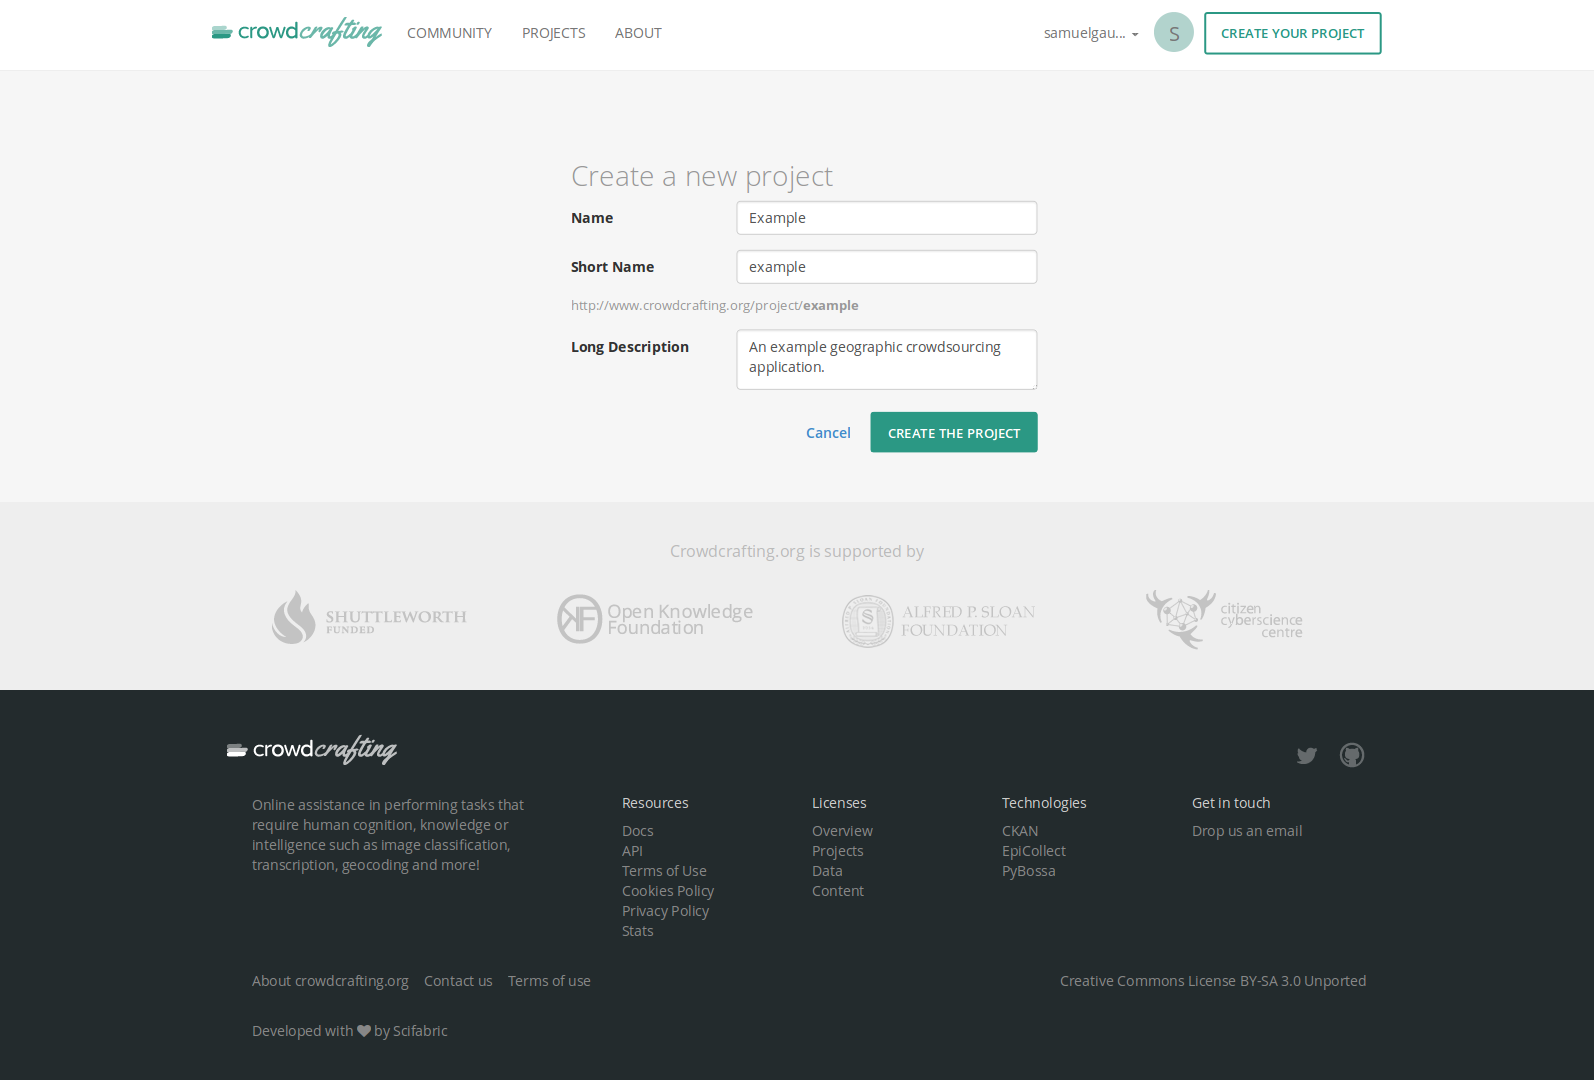
\includegraphics[width=4in]{cc-create}}
			\caption{Creating a project in \emph{crowdcrafting}}
			\label{fig:cc-create}
		\end{figure}

		\begin{figure}[ht]
			\centering
			\fbox{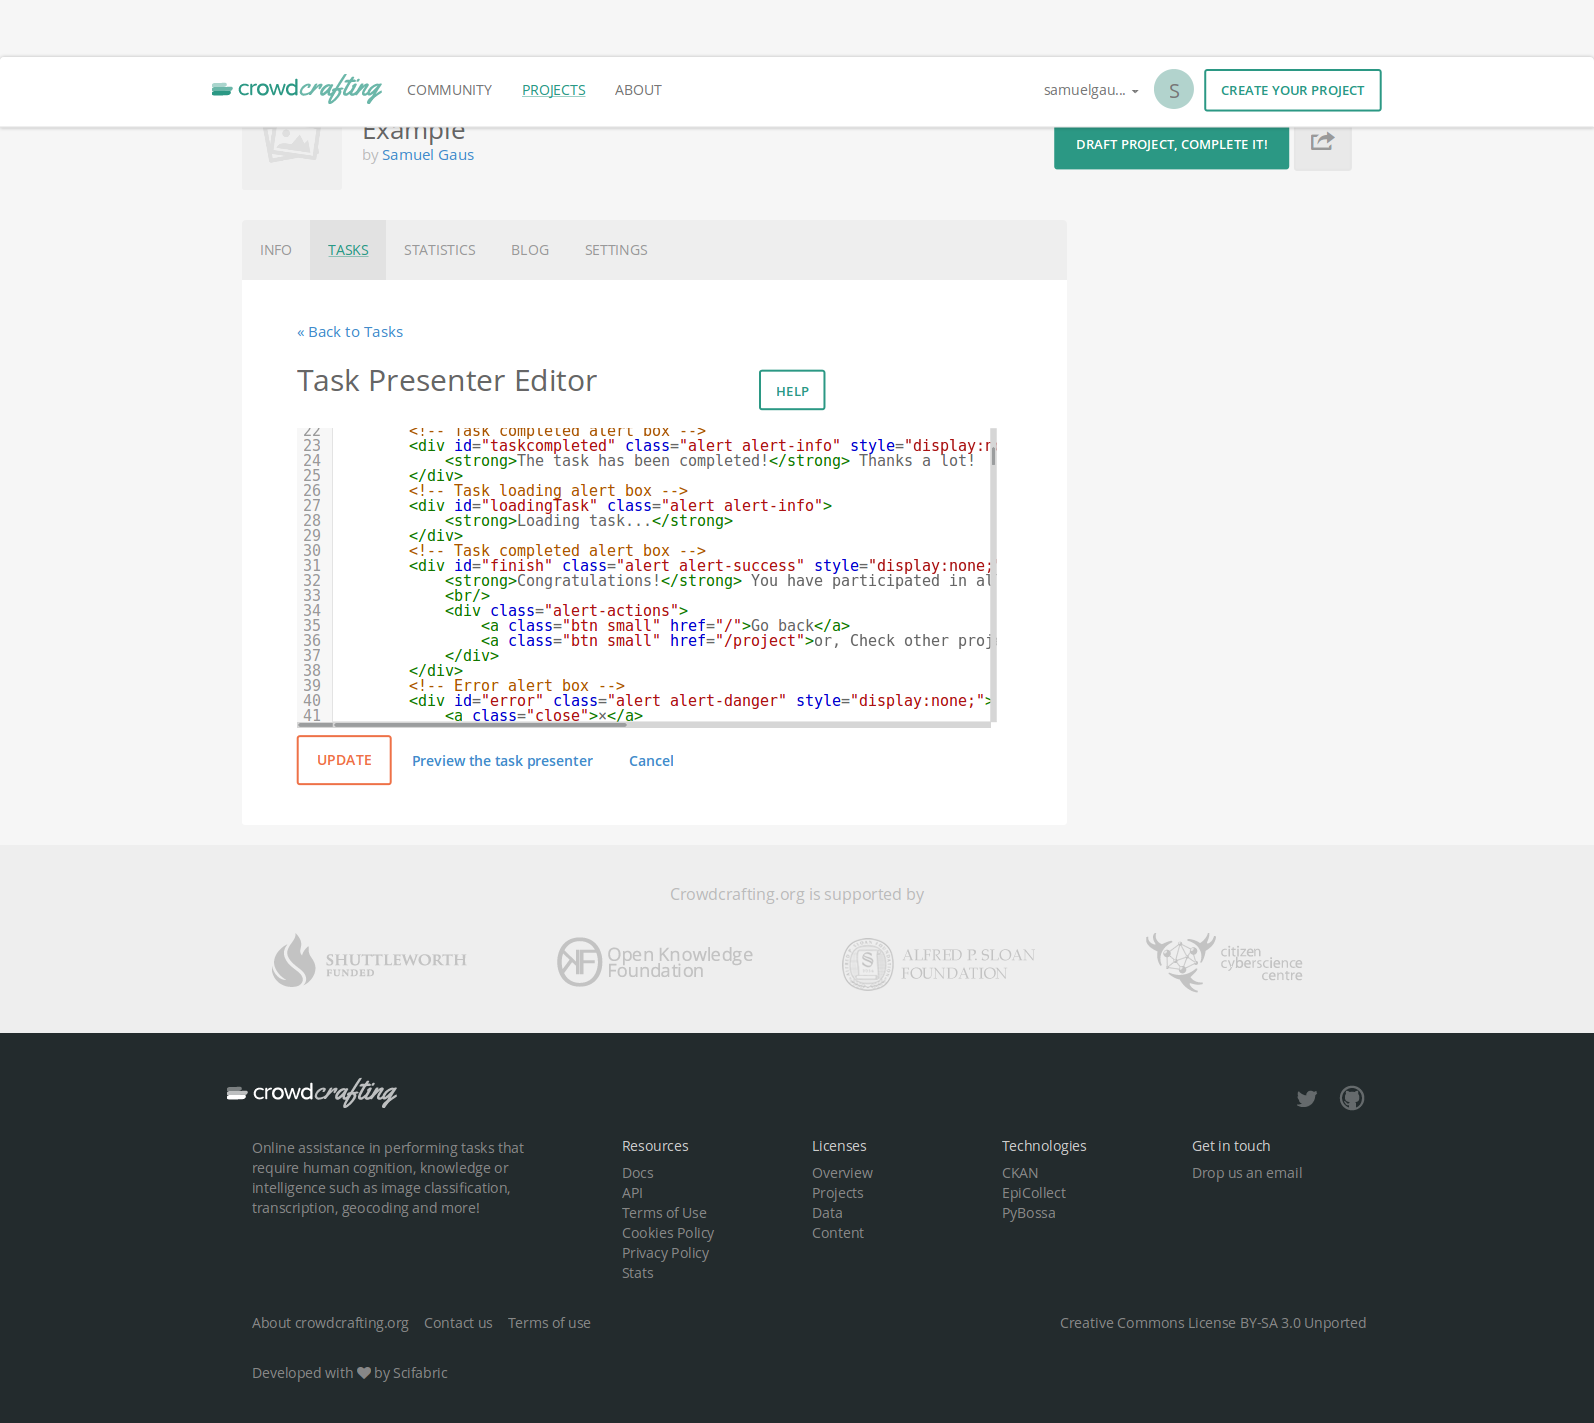
\includegraphics[width=4in]{cc-present}}
			\caption{Form creation screen in \emph{crowdcrafting}}
			\label{fig:cc-present}
		\end{figure}

		This would then create an input form for the data you wish to collect. However, because \emph{PyBOSSA} focusses on atomised tasks rather than a more general goal, it is not possible to create a question that any user can answer repeatedly. For example if you wanted to collect information about potholes, the task ``Where do you see a pothole?'' could be created. Once a user has `completed' this `task', however, they would not be able to answer it again, this causing the campaign to almost be one-use. Similarly, in the `Task Redundancy' settings area, you can specify how many times a single task can be repeated before closing. In the campaigns \emph{PyBOSSA} is built for, this would be to allow verification of submissions by seeing that multiple users provided the same data. In our example, however, it would be necessary to provide an arbitrary high number to allow the data collection to continue indefinitely.

		\subsubsection{FixMyStreet}

		\emph{FixMyStreet} is a much closer fit to the requirements in this study because it allows users to submit data on any location at a rate that they choose. Fortunately, the project is free\cite{_mysociety/fixmystreet_2015} and open source. However, the software itself is built specifically for reporting problems to a local authority and the back-end framework is very closely coupled with this concept and front-end. As a result, it would need heavy modification to work with a more generalised usage. This scale of modification required could be sufficient to justify building a new framework from the ground up, taking inspiration from \emph{FixMyStreet} rather than a straight fork of the codebase.

		\subsection{Conclusion}

		As was made clear when extracting the \hyperref[sec:common-functionalities]{common functionalities}, there is a huge overlap in the functionality of many crowdsourcing projects. There is a clear `type' of project for which a framework could be built that would save future campaign-creators having to make their own. This type of project - open submission of data with a geographic coordinate - is not well catered for by \emph{PyBOSSA}, which is built around finding a large task, atomising it into smaller tasks, and sharing them equally across the crowd. Even building something similar using \emph{PyBOSSA} would require significant technical knowledge to edit the \emph{HTML} and \emph{JavaScript} for the end-user to quickly enter data.

		A framework implementing the common functionalities could act as a level of abstraction away from these technical issues. From the analysis of the existing applications, a number of benefits can be drawn:

		\begin{enumerate}
			\pitem{Opening crowdsourcing to a wider audience} Currently there is some level of technical expertise required in setting up a crowdsourcing project of the type described. One either needs to be able to adapt existing open source technologies or write your own. Although this may be possible for some, it restricts the creation of crowdsourcing scenarios to those who have time and skill to dedicate to it.

			Crowdsourcing is meant to have the possibility of being casual - no one individual needs to carry the whole project because the data collection is shared by so many people. If this principal were applied to the creation of the campaign as well as the taking part, it's possible that much more data could be collected in general. Although this is not useful on its own clearly, if the collected data is open and available to the public it could be accessed easily by researchers. This is not without issue, however, as the casual nature of crowdsourcing has also been criticized academically\cite{brabham_myth_2012}.
			\pitem{Responding to time-critical data collection requirements} Even if one has the skill to apply to creating a crowdsourcing application to collect data, the campaign itself may be time critical. In a humanitarian crisis where data needs to be collected extremely quickly to be useful at all, it is much more preferable to have a system ready to be adapted to the specific needs and rolled out. For example, the usefulness of \emph{Tomnod} during the search for Malaysian Airlines Flight 370 would have been very little if it had come out several days later.
			\pitem{Saving money} A framework could save money for two reasons.
			\begin{itemize}
				\item Running and hosting pre-existing solutions costs money whereas a framework could offer a centralised platform (analogous to the relationship between \emph{PyBOSSA} and \emph{crowdcrafting}).
				\item These other problems can always be (and inevitably are) solved by spending money, either through hiring staff or learning new skills.
			\end{itemize}
			\pitem{Cross-pollination} If a centralised platform were hosted using this crowdsourcing platform, and they shared a web interface and mobile application, smaller campaigns would benefit for a number of reasons.
			\begin{itemize}
				\item Multiple campaigns could be accessed through the same interface. This means when a user is supplying information for a specific campaign of personal or public interest, they have the app open and would be more inclined to discover new campaigns.
				\item If a campaign is advertised to a user who already has the application installed on their phone, they may perceive the effort required as lower than it would be if they had to install a completely new application.
				\item Users could be emailed a newsletter featuring campaigns that they might find interesting, using collaborative or content-based filtering.
			\end{itemize}
		\end{enumerate}

	\section{Framework Design}
	\label{sec:architecture}
		As a result of the analysis and background above, a framework could be produced to provide sufficient functionality to replace the bespoke implementations so far. The framework would need to consist primarily of an API that can receive submitted data, perform all the necessary back-end organisation of that data, and expose a way of interacting with inbuilt data. On top of that, it will be necessary to construct a number of front-ends to interact with the API - a web-based and a mobile application.

		The \hyperref[sec:implementation]{next chapter} will cover the implementation of this design.

		\subsection{Requirements analysis}

		This section contains a detailed and quantifiable list of the requirements for the framework, built from the common functionalities of the analysed projects. To simplify accounting for each requirement in the implementation of the project, each requirement follows a continuous count, despite being split across categories.

		There are three data models around which the framework is based. Firstly, the User is the authenticated account and stable identity for anyone using the service. Although they are structurally the same, there are nonetheless two separate ``attitudes'' of User in the framework - campaign creators and campaign contributors. Throughout this section, where appropriate the requirements for each type will be differentiated with $\star$ for creator and $\dagger$ for contributor.

		Secondly, the Campaign is the name for the metadata around a campaign of data collection. For example, it contains a name for the campaign, a description of the data it is collecting and all other information about the campaign itself.

		Finally, the data that are contributed to Campaigns by Users are referred to as ``Points''.

		\newcounter{requirementcounter}
		\newcommand\rqrn{\stepcounter{requirementcounter}\arabic{requirementcounter}}

		\subsubsection{Users}

		\begin{table}[H]
			\begin{tabular}{ | l | l | l | }
				\hline
				\textbf{\textnumero} & \textbf{Sub-category} & \textbf{Requirement} \\ \hline\multicolumn{2}{| l }{} & \multicolumn{1}{ l | }{Users must be able to...}\\ \hline
				\rqrn & Authentication & Sign up.\\
				\rqrn & Authentication & Sign in.\\
				\rqrn & Authentication & Sign out.\\
				\rqrn & Authentication & Sign up and in using accounts from social media.\\
				\rqrn & Authentication & Reset their passwords.\\
				\rqrn & Authentication & Delete their accounts.\\
				\rqrn & Profiles & Edit their user profiles.\\
				\rqrn & Profiles & Find other users.\\
				\rqrn & Campaigns $\dagger$ & Join a campaign.\\
				\rqrn & Campaigns $\dagger$ & Leave a campaign.\\
				\rqrn & Campaigns $\star$ & Create a campaign.\\
				\hline
			\end{tabular}
			\caption{System requirements for management of Users.}
			\label{tab:reqs-users}
		\end{table}

		\subsubsection{Campaigns}

		\begin{table}[H]
			\begin{tabularx}{\textwidth}{ | l | l | X | }
				\hline
				\textbf{\textnumero} & \textbf{Sub-category} & \textbf{Requirement} \\ \hline
				\multicolumn{2}{| l }{} & \multicolumn{1}{ l | }{Campaigns must...}\\ \hline
				\rqrn & Design $\star$ & Be able to be created.\\
				\rqrn & Design $\star$ & Have names.\\
				\rqrn & Design $\star$ & Have a location.\\
				\rqrn & Design $\star$ & Allow the user creating them to provide a custom list of fields specific to their campaign.\\
				\rqrn & Design $\star$ & Support a start and end date outside of which they cannot receive data.\\
				\rqrn & Design $\star$ & Support a `text' field type.\\
				\rqrn & Design $\star$ & Support a `numerical' field type.\\
				\rqrn & Design $\star$ & Support a `boolean' field type.\\
				\rqrn & Design $\star$ & Support a `choose from a set of options' field type.\\
				\rqrn & Design $\star$ & Support an `image' field type.\\
				\rqrn & Design $\star$ & Be able to define `required' fields.\\
				\rqrn & Display & Be retrievable individually.\\
				\rqrn & Display & Be retrievable as a list.\\
				\rqrn & Display & Display associated points on a map, with icons or markers.\\
				\rqrn & Display $\dagger$ & Be searchable and sortable to assist in ``discovering'' new Campaigns.\\
				\rqrn & Administration $\star$ & Be updatable.\\
				\rqrn & Administration $\star$ & Be deletable.\\
				\rqrn & Administration $\star$ & Maintain a list of ``moderators'' - members with extra privileges to moderate content submitted.\\
				\rqrn & Administration $\star$ & Be able to be made private so that users must be invited rather than join freely.\\
				\rqrn & Administration $\star$ & Either be actively or passively moderated - i.e. data submissions join a queue to be approved, or are accepted and can be removed later.\\
				\rqrn & Administration $\star$ & Be able to give its Points a `shelf life', after which they become ``stale''.\\
				\hline
			\end{tabularx}
			\caption{System requirements for management of Campaigns.}
			\label{tab:reqs-campaigns}
		\end{table}

		\subsubsection{Points}

		\begin{table}[H]
			\begin{tabularx}{\textwidth}{ | l | l | X | }
				\hline
				\textbf{\textnumero} & \textbf{Sub-category} & \textbf{Requirement} \\ \hline
				\multicolumn{2}{| l }{} & \multicolumn{1}{ l | }{Points must...}\\ \hline
				\rqrn & Design $\dagger$ & Be able to be created and submitted to a Campaign of which the User is a member.\\
				\rqrn & Design $\dagger$ & Support a data payload that matches the schema of the Campaign \\
				\hline
			\end{tabularx}
			\caption{System requirements for management of Points.}
			\label{tab:reqs-points}
		\end{table}

		\subsection{Component architecture}

		\begin{figure}[ht]
			\centering
			\fbox{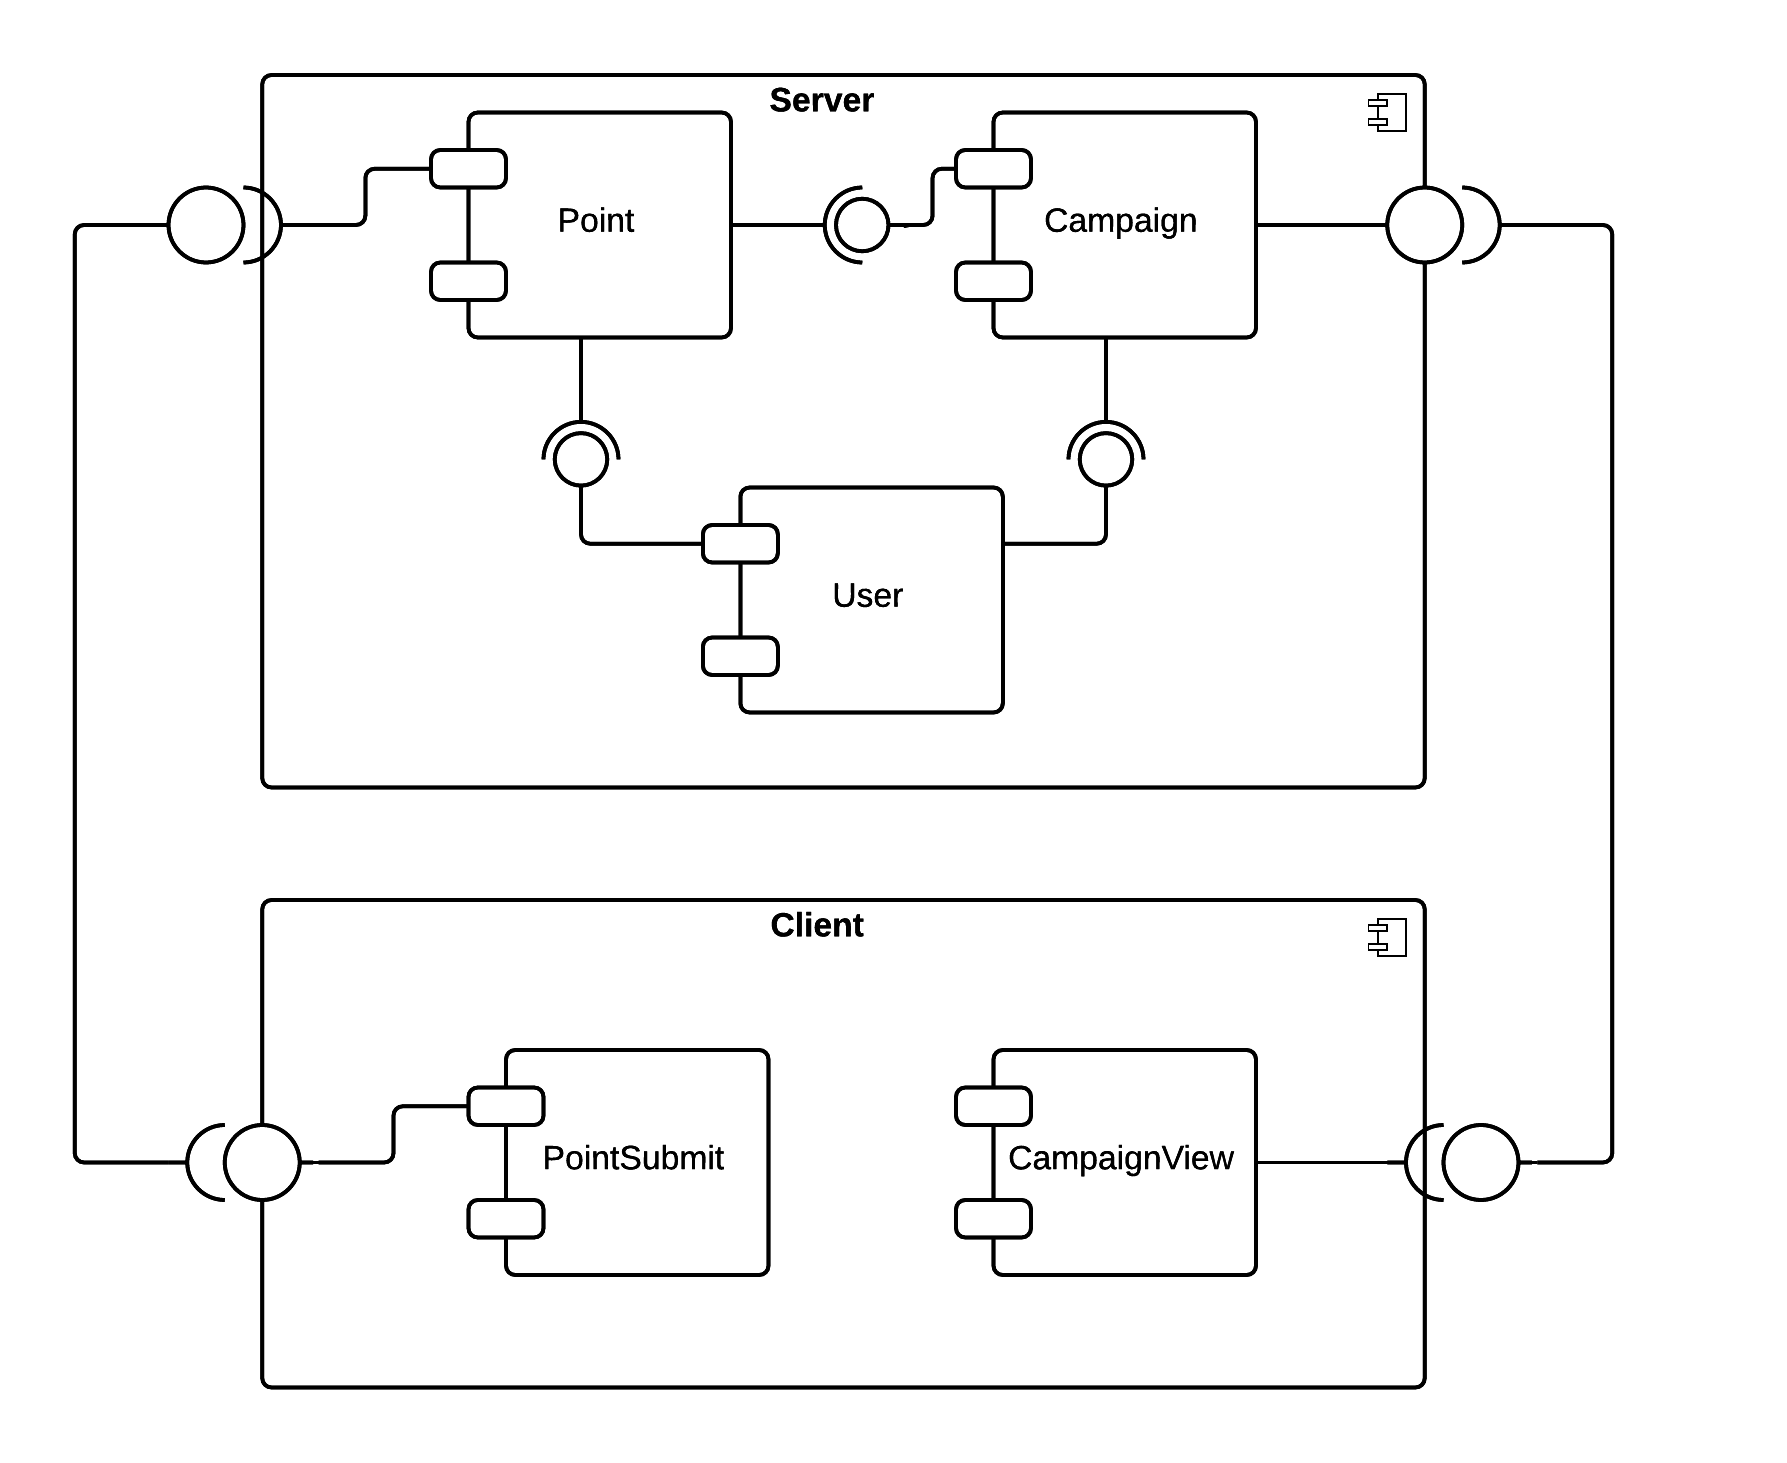
\includegraphics[width=4in]{component-diagram}}
			\caption{Component diagram}
			\label{fig:component-diagram}
		\end{figure}

		In Figure \ref{fig:component-diagram}, the relationship between components in the project is described. The framework follows a server-client architecture.

		\subsubsection{Server}

		The server carries out tasks like storing the data for the three models; validating submitted data; managing user authentication; and handling search queries. Instructions are provided using a REST (REpresational State Transfer) API over HTTP. REST over HTTP is an architectural style for semantic application interfaces. It leverages the ``methods'' defined in the specification for HTTP, and is recommended by the \emph{W3C}, who are in the draft stages of producing an official ``W3C Recommendation'' for its use\cite{_w3c_2012}.

		The data is split into three models - Campaigns, Points and Users. Users are the data model representing a user, which will contain authentication information. Campaigns are equivalent to a single project and represent a single campaign of data crowdsourcing. Users can join Campaigns and the submit Points, which will be related to a single campaign. A Point represents a single data item collected for a campaign and contains at least a geographic coordinate pair. A Point may also contain other information as detailed by the form structure set in the creation of a Campaign.

		API documentation can be found in \hyperref[sec:api-docs]{Appendix A}.

		\subsubsection{Client}

		The client comes in two forms - the web client and the mobile client. The key difference between the two is that the web client is served from a central server, whereas the mobile client is downloaded and stored on a mobile device.

		The client provides an interface for the user to interact with the framework by translating user actions into to find and join Campaigns, to see a list of the Campaigns that they have joined, to submit Points to a Campaign and to see a map of Points that have been submitted to a Campaign.

		A user can also create their own Campaign. A form is available that asks the user for the information required to create the Campaign, and the client transforms these options into an API request.

		\subsection{How it works}

		\subsubsection{Registering}
		To register, the user follows a link from the home page to a ``Sign up'' form, where they fill information such as their name, required username, email address and password. If the form has been filled in correctly, an account will be created for that user and they will be automatically logged in.

		\subsubsection{Creating a Campaign}
		To create a Campaign, a ``Create campaign'' link can be accessed from the home page, directing the user to a form with the necessary fields. The user selects a name for the Campaign, a central location and zoom level, a duration (if required), a time after which a submitted data point will go stale (if required), choose whether the Campaign is private to members only, if the campaign requires each point be approved by a moderator, and finally chooses the fields for the Campaign. The fields are chosen by adding as many fields as are required and selecting their ``type'' - boolean, numerical, text, multiple select or image. If the field is a multiple select, the user is further required to input different selections that can be made. An icon can be attached to each selection and, if required, the user can select that field's chosen option's icon be the marker on the resulting map for each point. Once submitted, the user will be brought to their new Campaign page, showing a blank map, the Campaign title and their name as the creator.

		\subsubsection{Discovering Campaigns}
		There is a page to ``View Campaigns'' even if the user is not a member, so new Campaigns can be discovered. At the top of the list are the Campaigns that the user has already joined. Below that, in a separate list, are all the Campaigns on the site that are not marked as ``private''. They are decorated with ``badges'' indicating whether they are ending soon, or whether the user is already a member.

		\subsubsection{Submitting information}
		To submit information to a Campaign, a specially emphasised button on the home page. This button leads the user to select from a list of Campaigns that they have joined. Once a Campaign is selected, the user is presented with a map on which to drop a pin, and the form specified by the Campaign creator. The user can choose to have the map automatically drop a pin based on their geolocation as reported by their browser or mobile device. Only once the map is marked and the form is filled out as specified in the creation of the campaign is the point submitted.

		\subsubsection{Browsing a Campaign}
		Clicking on a Campaign from the ``View Campaigns'' page brings you to the display page for that Campaign. The page features a map with all the points that have been submitted shown as markers (with an icon if specified). The map is centred to the configured ``centre point'' of the Campaign. The markers are clickable, and doing so leads the user to the full information attached to that Point.

		\subsubsection{Viewing a Point}
		When a marker is clicked, a page containing all the information for a Point is displayed. The page contains a map with just the marker visible, and a table of the information submitted along with the co-ordinate. If, for example, the information includes an uploaded picture, the picture will be visible in this table.

	\section{Implementation}
	\label{sec:implementation}

		The code is tracked using the \emph{Git} revision control system and is hosted on \emph{Github}. It can be found at \href{http://github.com/gausie/croud}{\nolinkurl{http://github.com/gausie/croud}}. The software is also running and available to be used at \href{http://croud.io}{\nolinkurl{http://croud.io}}.

		Due to the quantity of code across a wide directory structure, the source code is not included as an appendix. Instead, this section will cover some highlights of code behind the key functionalities.

		\subsection{Technologies}

		The server is written using \emph{JavaScript}, running server-side using \emph{Node.js}. This the software being primarily event-driven (i.e. responding to events rather than running tasks constantly) and potentially requiring a high volume of concurrent users\cite{tilkov_node.js:_2010}. Because the platform is designed to support multiple Campaigns being run simultaneously, the software needs to be scalable. This language was also chosen due to developer preference and the current proliferation of third-party libraries available in the \emph{JavaScript} ecosystem. In particular, the application was scaffolded using \emph{MEAN.JS}, a bootstrap for applications using a ``MEAN'' stack - or \emph{MongoDB}, \emph{express}, \emph{AngularJS} and \emph{Node.js}.

		Within the \emph{Node.js} environment, the \emph{express} framework is used to wrap the HTTP server, and \emph{passport} is used to handle multiple login strategies (local or via social media accounts).

		For storing data, the software uses the document-oriented database \emph{MongoDB}. This is beneficial for this system for a number of reasons, listed below.

		\begin{itemize}
			\item The data's interrelationship is not complex and can easily be handled by the basic \emph{MongoDB} table relationship schema.
			\item Dynamic schemas are extremely useful in storing Points because each Campaign can require a different data structure to be collected per point. In a relational \emph{SQL}-based database this would be complicated, requiring another table to store the fields. On \emph{MongoDB}, however, it is an extremely trivial issue.
			\item The support for geographic data is good, with the ability to query coordinate data on a simulated 2d sphere extremely quickly.
			\item \emph{MongoDB} can very quickly be scaled to run in a distributed manner from a number of machines. This is useful for saving money in a cloud environment where the software can quickly scale up depending on usage.
		\end{itemize}

		The client software is written in \emph{HTML} and JavaScript, using the \emph{AngularJS} MVC application framework. This was chosen because of widespread usage resulting in third-party libraries, and developer experience. The mobile application is produced from bundling the web application using \emph{Cordova}, a mobile development framework produced by \emph{Apache} allowing the creation of native mobile applications using \emph{HTML} and \emph{JavaScript}.

		The software is designed to run on any operating system, but in the current production environment is running on a \emph{Linux} server provided by \emph{Heroku}.

		\subsection{Schema}

		As \emph{MongoDB} uses dynamic schemas, these are not necessarily how documents stored in each collection might look. Instead, the schema here is the framework of a model described in JavaScript, and as a result contains some callbacks as values (which would not be valid in plain JSON).

		\subsubsection{User}

		\begin{minted}[frame=single,fontsize=\scriptsize]{js}
{
  firstName: {
    type: String,
    trim: true,
    default: '',
    validate: [validateLocalStrategyProperty, 'Please fill in your first name']
  },
  lastName: {
    type: String,
    trim: true,
    default: '',
    validate: [validateLocalStrategyProperty, 'Please fill in your last name']
  },
  displayName: {
    type: String,
    trim: true
  },
  email: {
    type: String,
    trim: true,
    default: '',
    validate: [validateLocalStrategyProperty, 'Please fill in your email'],
    match: [/.+\@.+\..+/, 'Please fill a valid email address']
  },
  username: {
    type: String,
    unique: 'testing error message',
    required: 'Please fill in a username',
    trim: true
  },
  password: {
    type: String,
    default: '',
    validate: [validateLocalStrategyPassword, 'Password should be longer']
  },
  memberships: [{
      type: Schema.ObjectId,
      ref: 'Campaign',
  }],
  salt: {
    type: String
  },
  provider: {
    type: String,
    required: 'Provider is required'
  },
  providerData: {},
  additionalProvidersData: {},
  roles: {
    type: [{
      type: String,
      enum: ['user', 'admin']
    }],
    default: ['user']
  },
  updated: {
    type: Date
  },
  created: {
    type: Date,
    default: Date.now
  },
  /* For reset password */
  resetPasswordToken: {
    type: String
  },
  resetPasswordExpires: {
    type: Date
  }
}
		\end{minted}

		\subsubsection{Campaign}

		\begin{minted}[frame=single,fontsize=\scriptsize]{js}
{
  name: {
    type: String,
    default: '',
    required: 'Please fill Campaign name',
    trim: true
  },
  location: {
    lng: { type: Number },
    lat: { type: Number },
    zoom: { type: Number }
  },
  locationArray: {
    type: [Number],
    index: '2dsphere'
  },
  fields: {
    type: Schema.Types.Mixed
  },
  duration: {
    start: {
      type: Date
    },
    end: {
      type: Date
    }
  },
  private: {
    type: Boolean,
    default: false
  },
  approvalRequired: {
    type: Boolean,
    default: false
  },
  fieldAsMarker: {
    type: String
  },
  stale: {
    type: Number
  },
  created: {
    type: Date,
    default: Date.now
  },
  user: {
    type: Schema.ObjectId,
    ref: 'User'
  }
}
		\end{minted}

		The ``fields'' field is a JSON sub-structure built from the data required for each campaign. For example, it could contain a value such as

		\begin{minted}[frame=single,fontsize=\scriptsize]{json}
[
    {
        "options" : [ 
            {
                "icon" : "gamepad",
                "name" : "Water"
            }, 
            {
                "icon" : "search",
                "name" : "Toll Both"
            }
        ],
        "required" : true,
        "type" : "select",
        "name" : "Point of Interest"
    },
    {
        "required" : false,
        "type" : "image",
        "name" : "Picture"
    }
]
		\end{minted}

		\subsubsection{Point}

		\begin{minted}[frame=single,fontsize=\scriptsize]{js}
{
  campaign: {
    type: Schema.ObjectId,
    ref: 'Campaign'
  },
  location: {
    lat: { type: Number },
    lng: { type: Number }
  },
  locationArray: {
    type: [Number],
    index: '2dsphere'
  },
  data: {
    type: Schema.Types.Mixed
  },
  approved: {
    type: Boolean,
    default: true
  },
  created: {
    type: Date,
    default: Date.now
  },
  user: {
    type: Schema.ObjectId,
    ref: 'User'
  }
}
		\end{minted}

		The ``data'' field is a JSON sub-structure matching the ``fields'' field of the Campaign to which the Point belongs. For example, it could contain a value such as

		\begin{minted}[frame=single,fontsize=\scriptsize]{json}
{
    "Point of Interest" : {
        "icon" : "gamepad",
        "name" : "Water"
    }
}
		\end{minted}

		\subsection{Code excerpts}

		This section will contain a few examples of the source code and is not intended to be exhaustive.

		\subsubsection{Server}

		\paragraph{Querying points}

		\begin{minted}[frame=single,linenos,fontsize=\scriptsize]{js}
/**
 * List of Points
 */
exports.list = function(req, res) {
  var query = Point.find();

  // Filter Points by campaign, else populate with the campaign details.
  if (req.query.campaign) {
    query.where('campaign').equals(req.query.campaign);
  } else {
    query.populate('campaign');
  }

  // Filter points by user
  if (req.query.user) {
    query.where('user').equals(req.query.user);
  }

  //  Only return Points within a certain bounds if needed.
  if (req.query.bounds) {
    var b = req.query.bounds.split(',');
    query.where('locationArray').within().box(b.slice(0,2), b.slice(2,4));
  }

  query.sort('-created').populate('user', 'displayName').exec(function(err, points) {
    if (err) {
      return res.status(400).send({
        message: errorHandler.getErrorMessage(err)
      });
    } else {
      res.jsonp(points);
    }
  });
};
	\end{minted}

	This section of code is the callback for the controller handling \texttt{GET} requests to \texttt{/points} endpoint. The Point variable is an object referring to a MongoDB class (using the \emph{Mongoose} JavaScript library), and it is instantiated to \texttt{query} using the \texttt{find()} method with no arguments. Different HTTP query parameters are appended to the \texttt{req} argument by \emph{express}. If they are found to exist in this callback, they alter the \texttt{query} object by reference.

	For example, if we are looking for Points in a specific Campaign, we add chain the \texttt{where} and \texttt{equals} methods (lines~8-10,) 		 which is syntactical sugar for \emph{mongoose} to add our conditions to the query it is building. The benefit of building queries in this way is that it means the system is not vulnerable to an injection attack, where a maliciously crafted query could break out of the execution context within which it is intended to operate and affect other parts of the database or code.

	Also to be noted here is the simplicity with which \emph{MongoDB} (and, in turn, \emph{mongoose}) deal with geographical queries. On line~22 the \texttt{within} and \texttt{box} methods are chained to quickly define a fence within which we want our Points to be.

	\paragraph{Deleting a Campaign}

	\begin{minted}[frame=single,linenos,fontsize=\scriptsize]{js}
/**
 * Delete an Campaign.
 *
 * Also unjoins all joined Users.
 */
exports.delete = function(req, res) {
  var campaign = req.campaign;

  // Start an object of tasks to be carried out.
  var tasks = {};

  // Delete the campaign.
  tasks.campaign = function(done) {
    campaign.remove(function(err, result) {
      done(err, result);
    });
  };

  User.findUsersInCampaign(campaign, function(err, users) {
    if (err) {
      return res.status(400).send({
        message: errorHandler.getErrorMessage(err)
      });
    } else {
      // Add task to leave every joined user from the group.
      users.forEach(function(user) {
        tasks[user._id] = function(done) {
          user.leaveCampaign(campaign, function(err, result) {
            done(err, result);
          });
        };
      });

      // Carry out all the tasks in parallel.
      async.parallel(tasks, function(err, results) {
        if (err) {
          return res.status(400).send({
            message: errorHandler.getErrorMessage(err)
          });
        } else {
          res.jsonp(results.campaign);
        }
      });
    }
  });

};
	\end{minted}

	This section of code is the callback for the controller handling \texttt{DELETE} requests to \texttt{/campaigns/:campaignId} endpoints. Note that this occurs after middleware that checks whether a user is authenticated to carry out the command.

	The Campaigns of which a User is a member is stored in a collection on the User object. \emph{MongoDB} is not a relational database and so the data is stored in this way to be fastest - most of the time we need to know what Campaigns a User is a member of, rather than know what Users are members of a campaign (although this would also be trivial to calculate). The only added complication is that when a Campaign is deleted, every member needs to remove it from their membership list. Because of the asynchronous nature of a number of the requests carried out by this function, instead of carrying out each instruction in sequence the callbacks required are collected in an object called \texttt{tasks}. Once the tasks are all collected, the \emph{async} library is used to execute them all in parallel (line~35) and send a response to the client once complete.

	\paragraph{Authorization Middleware}

	\begin{minted}[frame=single,linenos,fontsize=\scriptsize]{js}
app.route('/campaigns/:campaignId')
  .delete(users.requiresLogin, campaigns.hasAuthorization, campaigns.delete);
	\end{minted}

	\begin{minted}[frame=single,linenos,fontsize=\scriptsize]{js}
exports.hasAuthorization = function(req, res, next) {
  if (req.campaign.user.id !== req.user.id) {
    return res.status(403).send('User is not authorized');
  }
  next();
};
	\end{minted}

	This is an example of authorization middleware. The first snippet is an \emph{express} routing expression, listing a chain of callbacks to process on a \texttt{DELETE} request to \texttt{/campaigns/:campaignId}. The second callback (line~2) \texttt{campaigns.hasAuthorization} can be seen in the second snippet. The \texttt{req} variable has been populated with \texttt{campaign} and \texttt{user} from middleware elsewhere in the application. On line~2 the campaign owner and authenticated user are compared, but if they are indeed equal, the \texttt{next} function passes control to the next middleware callback.

	\subsubsection{Client}

	Because the client is written using \emph{AngularJS}, which spreads the implementation across the views and controllers, code snippets will not be as fluid as in the Server section.

	\paragraph{Campaign field design}

	\subparagraph{View}
	\inputminted[frame=single,linenos,breaklines,fontsize=\scriptsize]{xml}{snippets/campaign-field-design.html}
	Note: this is trimmed down from the true source to save space.

	\subparagraph{Controller}
	\inputminted[frame=single,linenos,breaklines,fontsize=\scriptsize]{js}{snippets/campaign-field-design.js}

	\emph{AngularJS} has the ability to repeat HTML elements based on objects attached to \texttt{\$scope}. In this example, the \texttt{fields} object populates the form's input fields using the \texttt{addField} and \texttt{removeField} functions. Within each field, there is an option to use the type multiple choice ``select'' type, and options can be added and removed using the \texttt{addOption} and \texttt{removeOption} functions.

	Options for a ``select'' type come with icons, which are loaded from a list generated from the icons available in the \emph{FontAwesome} icon pack. The ``Use field as marker'' option can only be selected in one field and, if checked, will replace the generic markers on the Campaign's display map with the icon selected in the point submitted.

	\subsection{Features}

	Although the framework is useful for starting campaigns in any case, there are a number of features implemented that are non-trivial to produce. Were a developer to create a framework from scratch, the basic data storage might come quickly, but these features would encourage developers to use pre-existing software. Below are listed a few of these features.

	\paragraph{Points going stale}
	In this framework, it's possible to mark Campaigns with the property of their Points expiring or going ``stale'' after a set amount of time. This feature is useful for Campaigns collecting information that is time sensitive and not relevant if it hasn't been recently submitted. This is common in humanitarian crowdsourcing campaigns. At the moment, being stale just visually distinguishes the Point when it is being displayed on a map, but in the future the feature could be expanded upon. For example, users could be reminded to re-check their stale submissions; or Users who submitted data nearby could be asked if they would like to help out.

	\paragraph{Customizable Campaign field schemas}
	As covered partly in one of the code snippets above, the framework is capable of handling any number of typed (and thus validatable) fields. There are five field types to choose from: boolean, numerical, text, multiple choice and file. Any number of these fields can be added to a Campaign in any configuration, with the creator being able to specify whether they are required or not, and if the icon chosen in the multiple choice field should be used as the map marker.

	\paragraph{Standards-compliant mobile-ready client}
	The client is written in a fully standards-compliant fashion and the display completely adapts to mobile. This means that the web version is viewable on a wide range of browsers, usable by users with accessibility requirements such as the use of a screen-reader. It also means that the web version can be viewed on mobiles and tablets with a fluid experience. This is useful also in packaging the client as a native mobile application, as very little changes need to be made and so changes to the codebase can be quickly expanded across the whole ecosystem.

	\section{Evaluation}
	\label{sec:evaluation}

		In evaluating the framework, it is necessary to test two aspects of the framework's usage - the creation of Campaigns, and the submission of points. In this section, a number of key features will be tested by using the software and providing screenshots and comments. First, the client will be used to create two Campaigns that are as distinct as possible in usage scenarios. These campaigns will be

		\begin{enumerate}[label=\Alph*.]
			\item A humanitarian Campaign similar to the \emph{Missing Maps} project. The campaign is designed to collect time-sensitive information about the physical environment, and as a result will have a time limit after which a Point will be marked stale. It will be a private campaign open only to invited members.
			\item A simple ``fix this pothole'' style project where users casually submit images with location data. The campaign will be open to all to join.
		\end{enumerate}

		Using a second account, the second Campaign will be joined and a point will be submitted.

		\subsection{Preparing users}

		\begin{figure}[ht]
			\centering
			\fbox{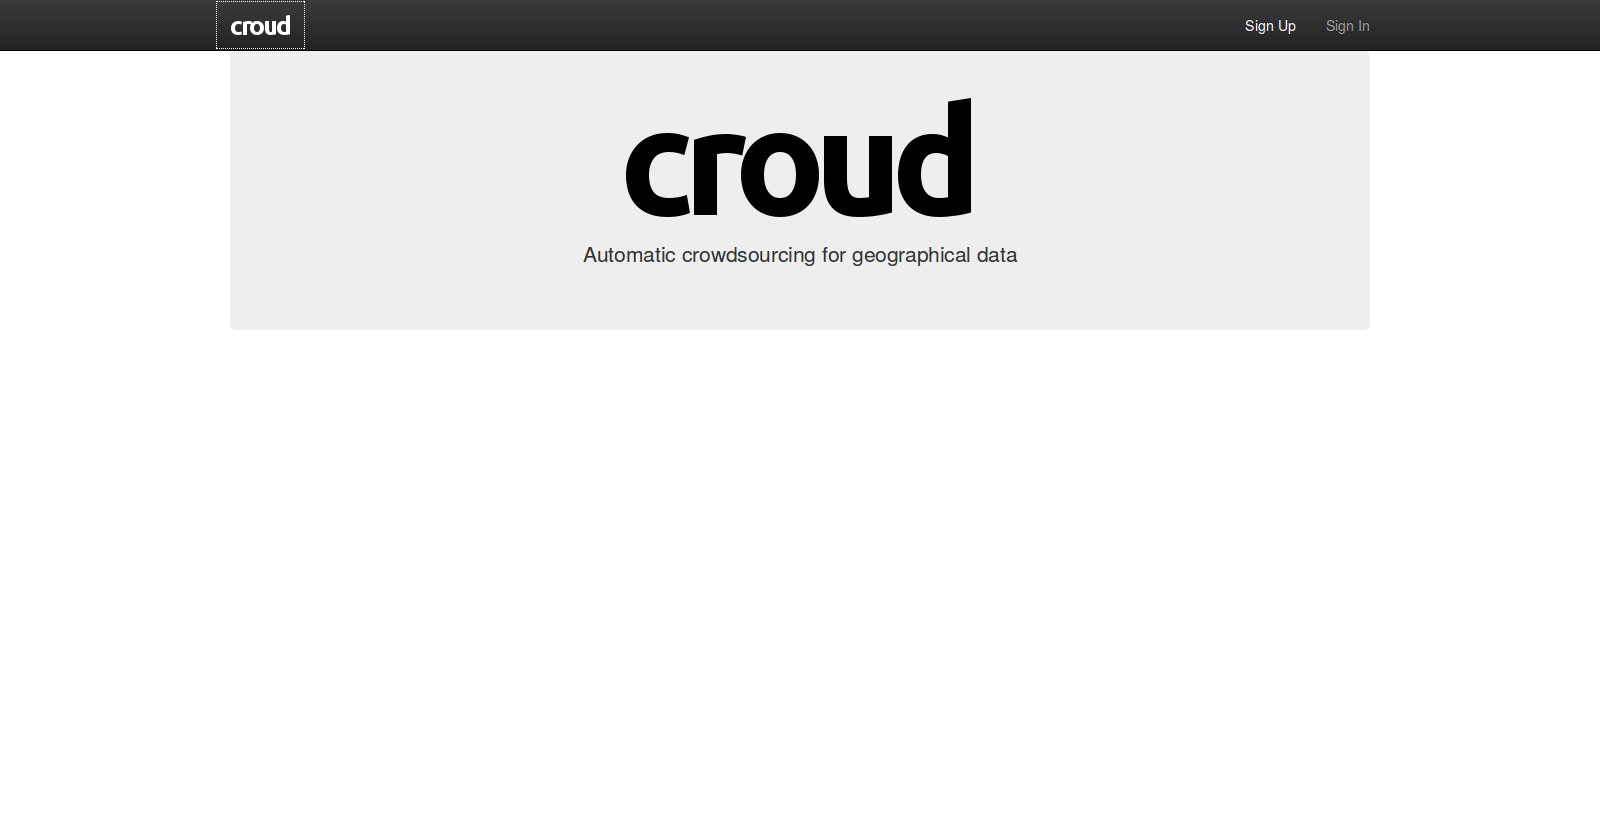
\includegraphics[width=4in]{eval-prep-1}}
			\caption{Landing page}
			\label{fig:eval-prep-1}
		\end{figure}

		\begin{figure}[ht]
			\centering
			\fbox{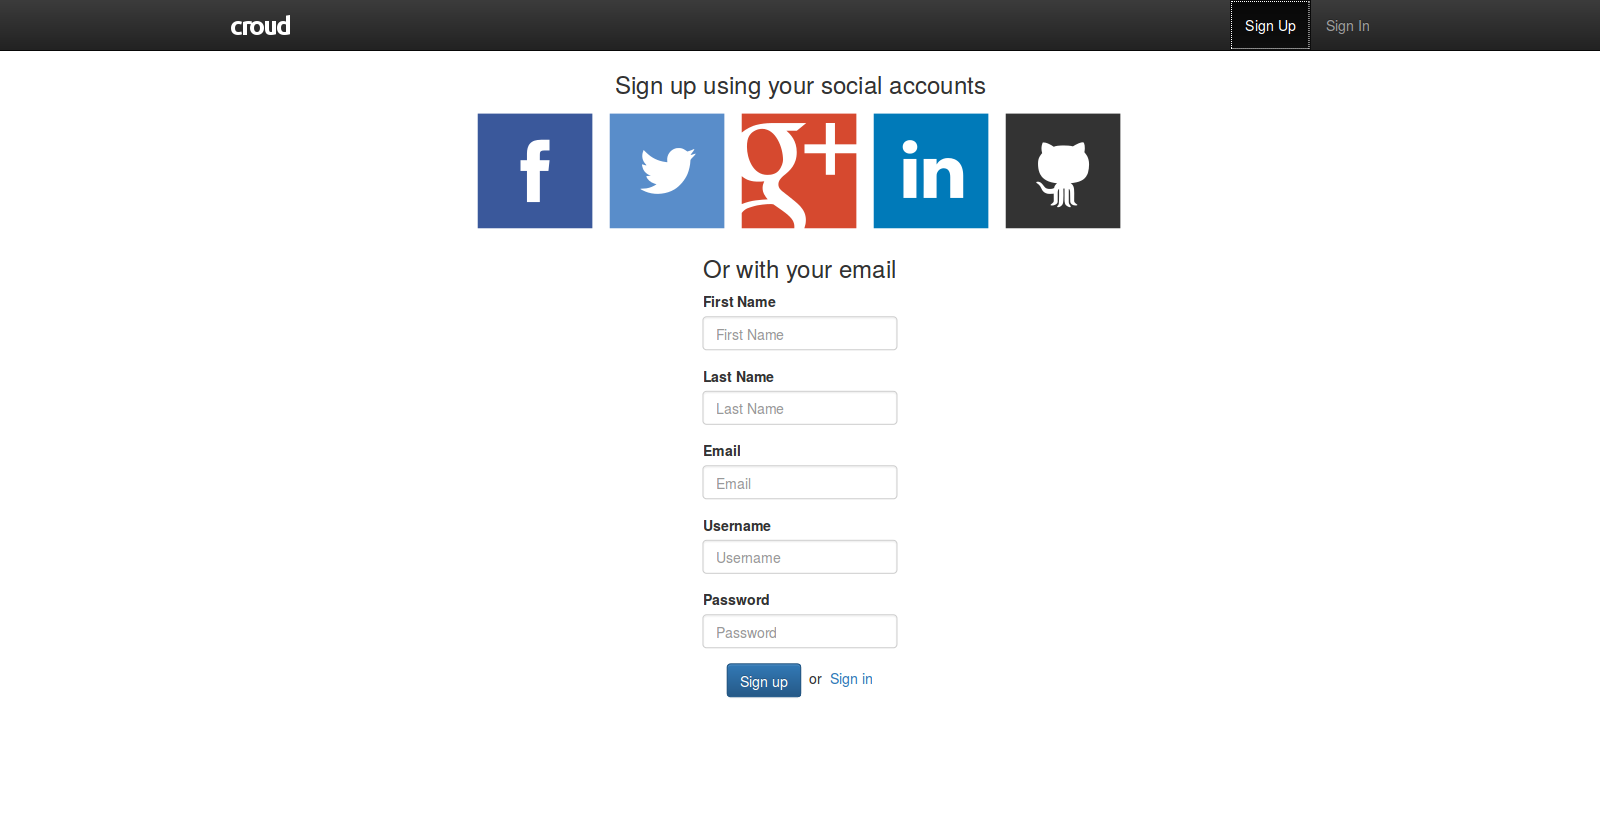
\includegraphics[width=4in]{eval-prep-2}}
			\caption{Registration page.}
			\label{fig:eval-prep-2}
		\end{figure}

		\begin{figure}[ht]
			\centering
			\fbox{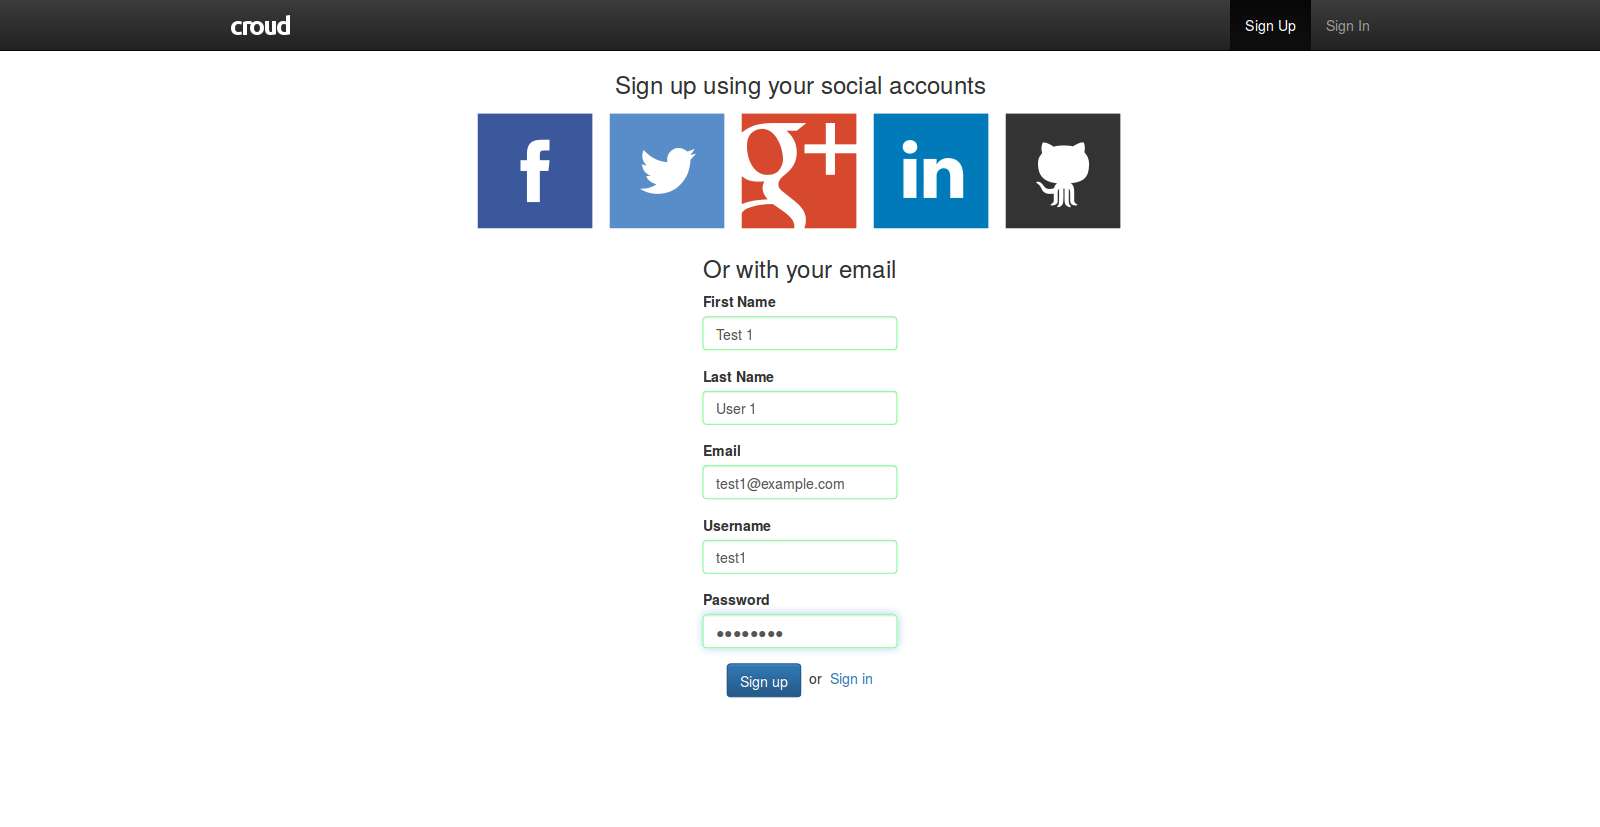
\includegraphics[width=4in]{eval-prep-3}}
			\caption{Registering \texttt{test1} user.}
			\label{fig:eval-prep-3}
		\end{figure}

		\begin{figure}[ht]
			\centering
			\fbox{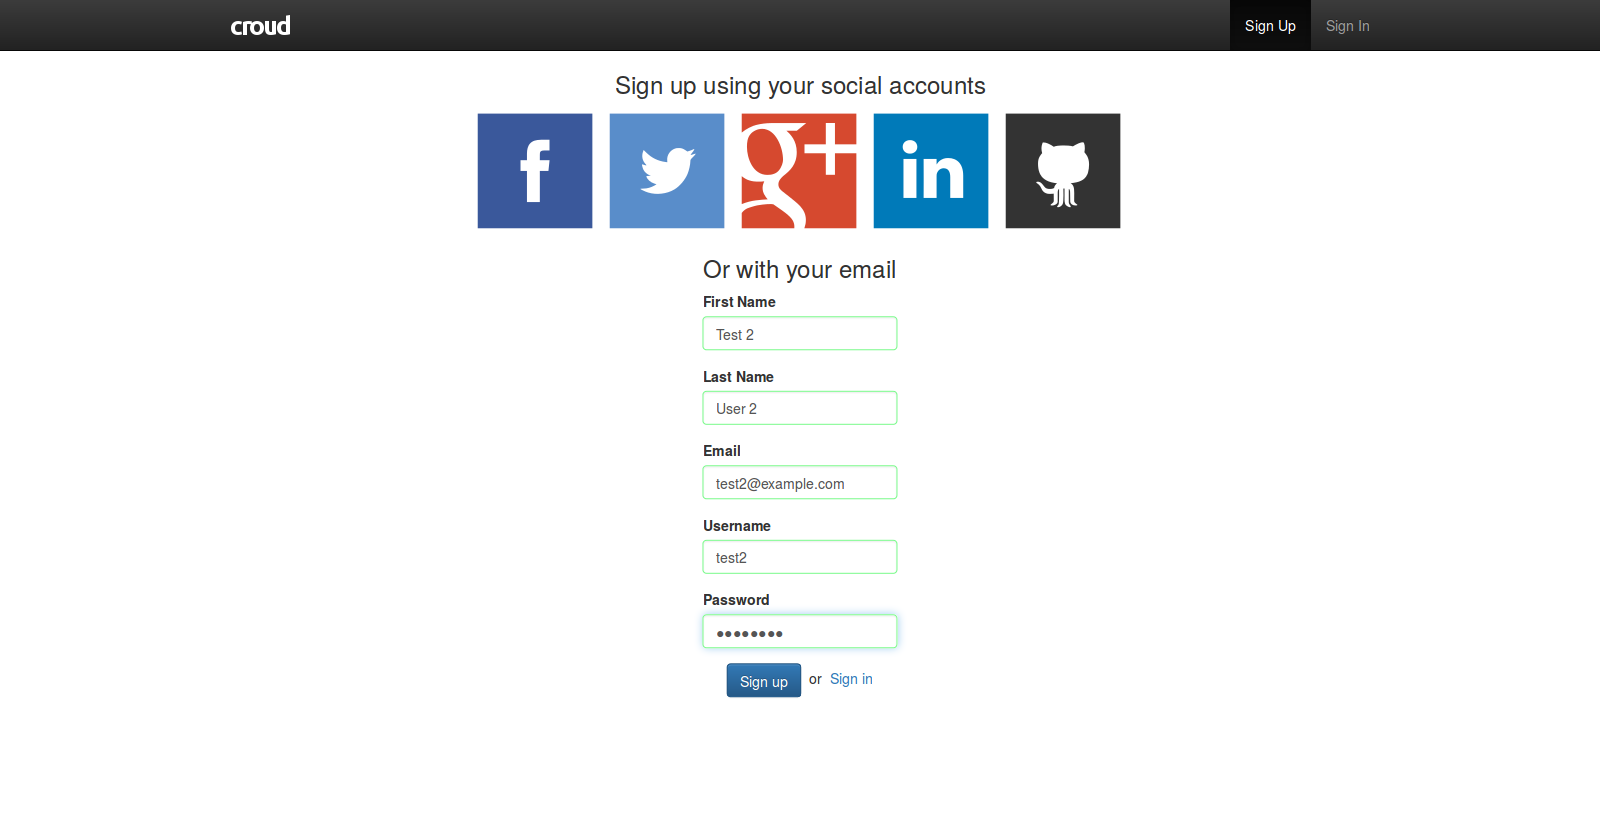
\includegraphics[width=4in]{eval-prep-4}}
			\caption{Registering \texttt{test2} user.}
			\label{fig:eval-prep-4}
		\end{figure}

		\FloatBarrier
		\subsection{Creating Campaign A}

		\begin{figure}[ht]
			\centering
			\fbox{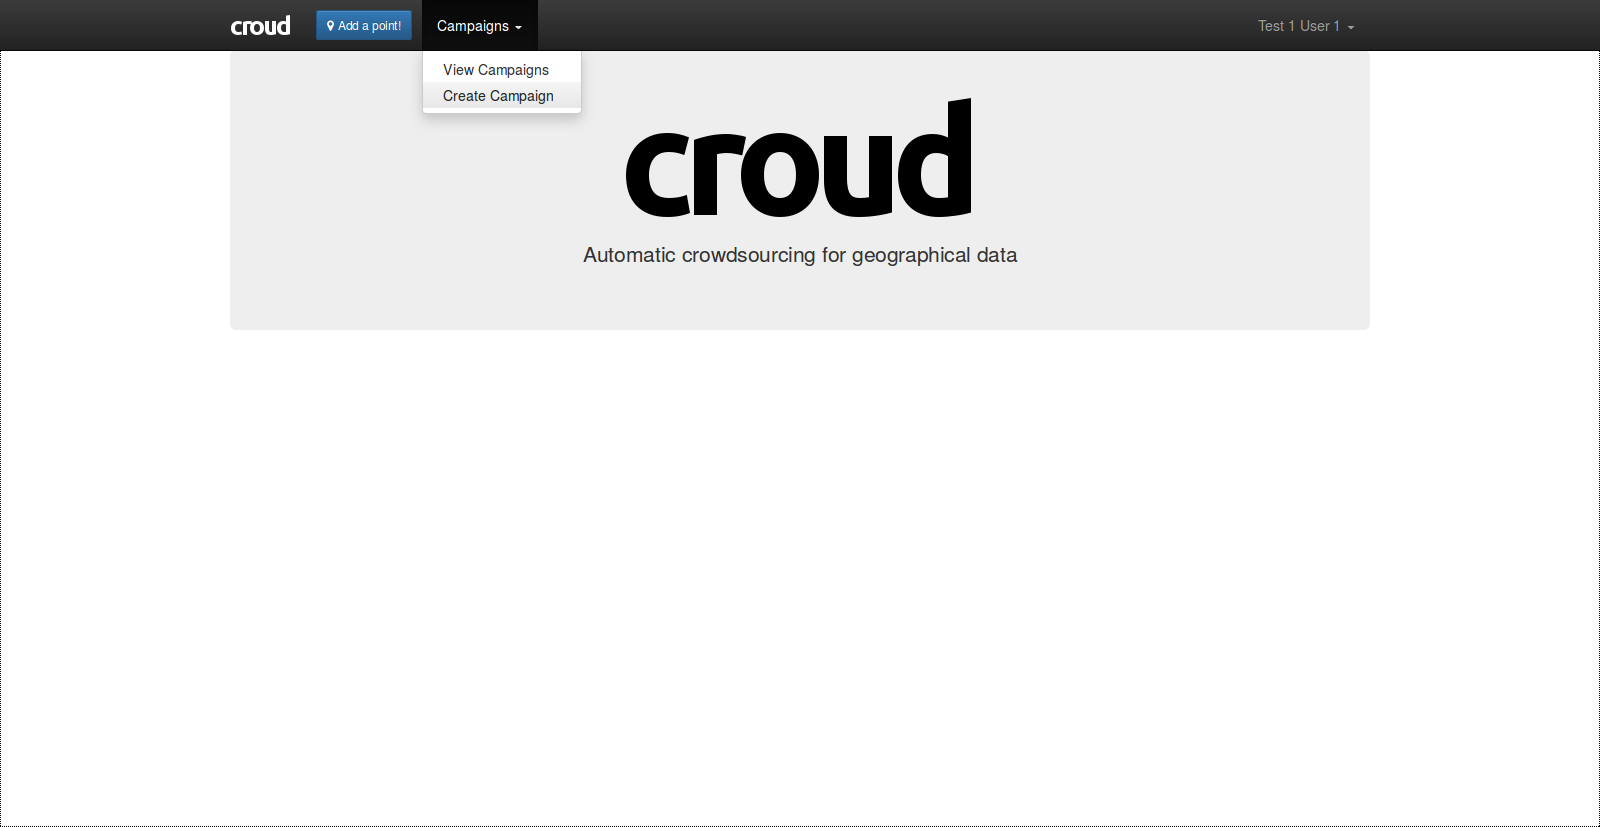
\includegraphics[width=4in]{eval-ca-1}}
			\caption{Navigating to Campaign creation page.}
			\label{fig:eval-ca-1}
		\end{figure}

		\begin{figure}[ht]
			\centering
			\fbox{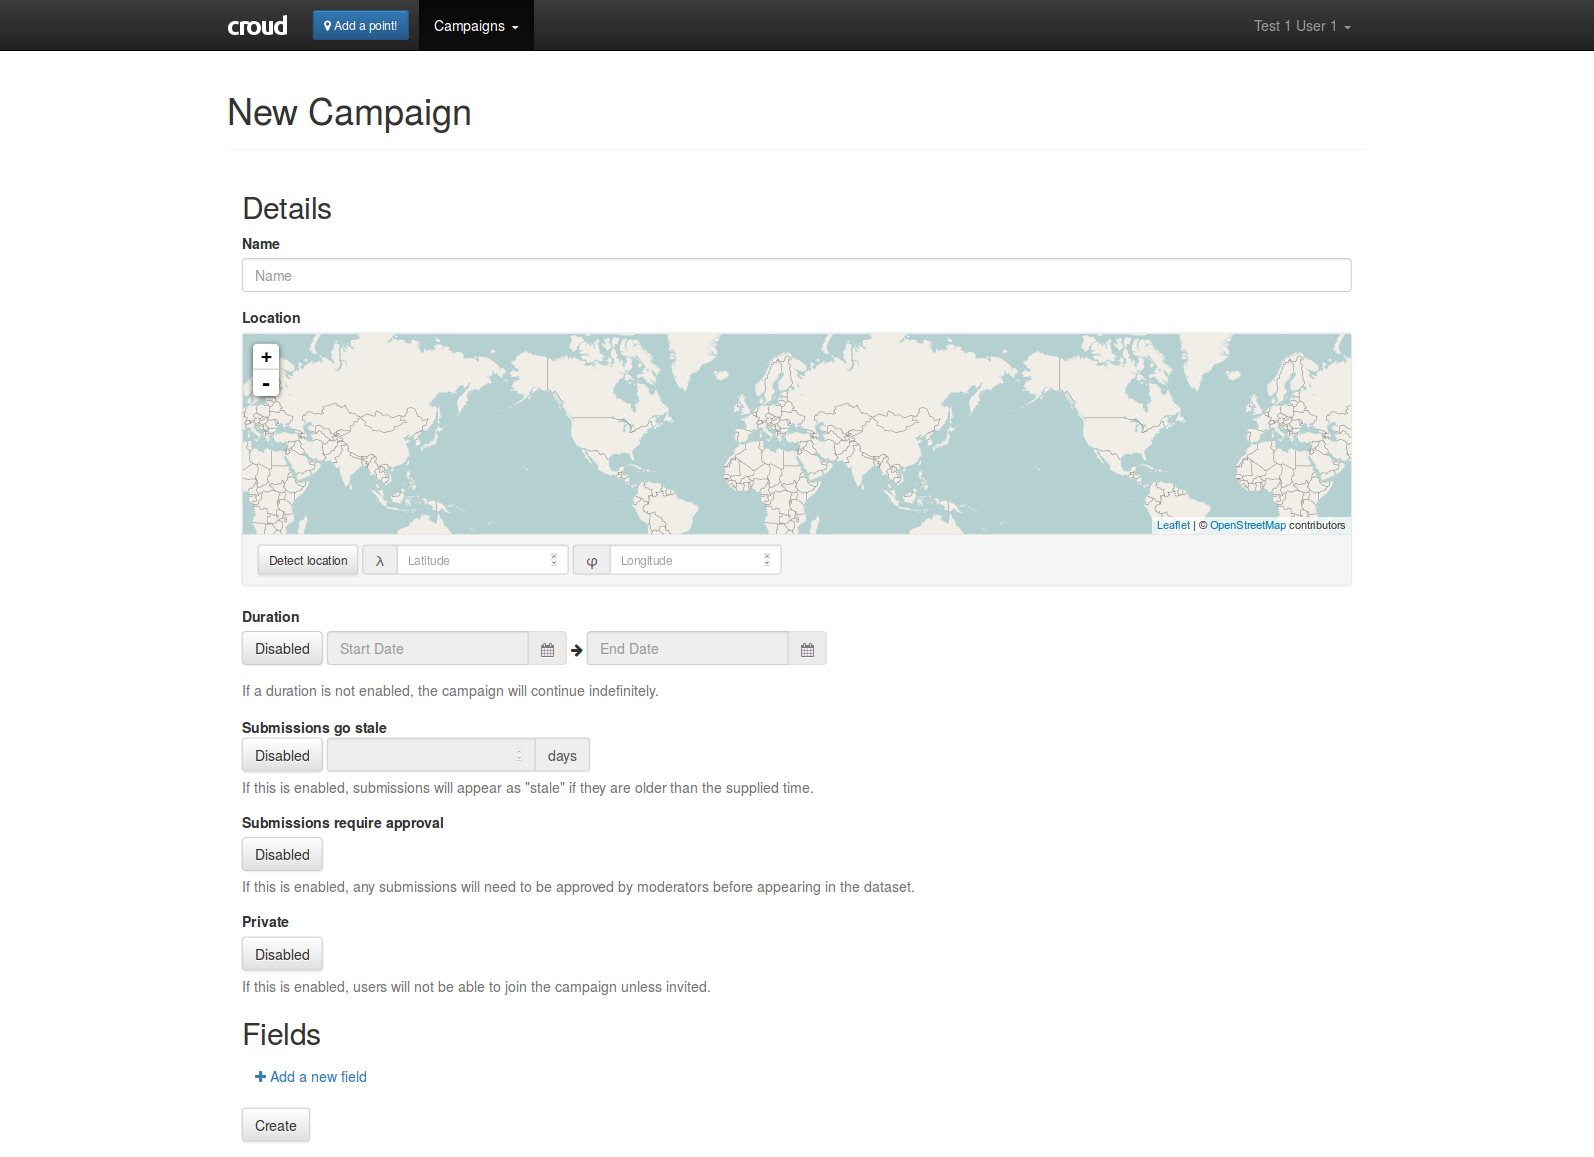
\includegraphics[width=4in]{eval-ca-2}}
			\caption{Initial state of Campaign creation form.}
			\label{fig:eval-ca-2}
		\end{figure}

		\begin{figure}[ht]
			\centering
			\fbox{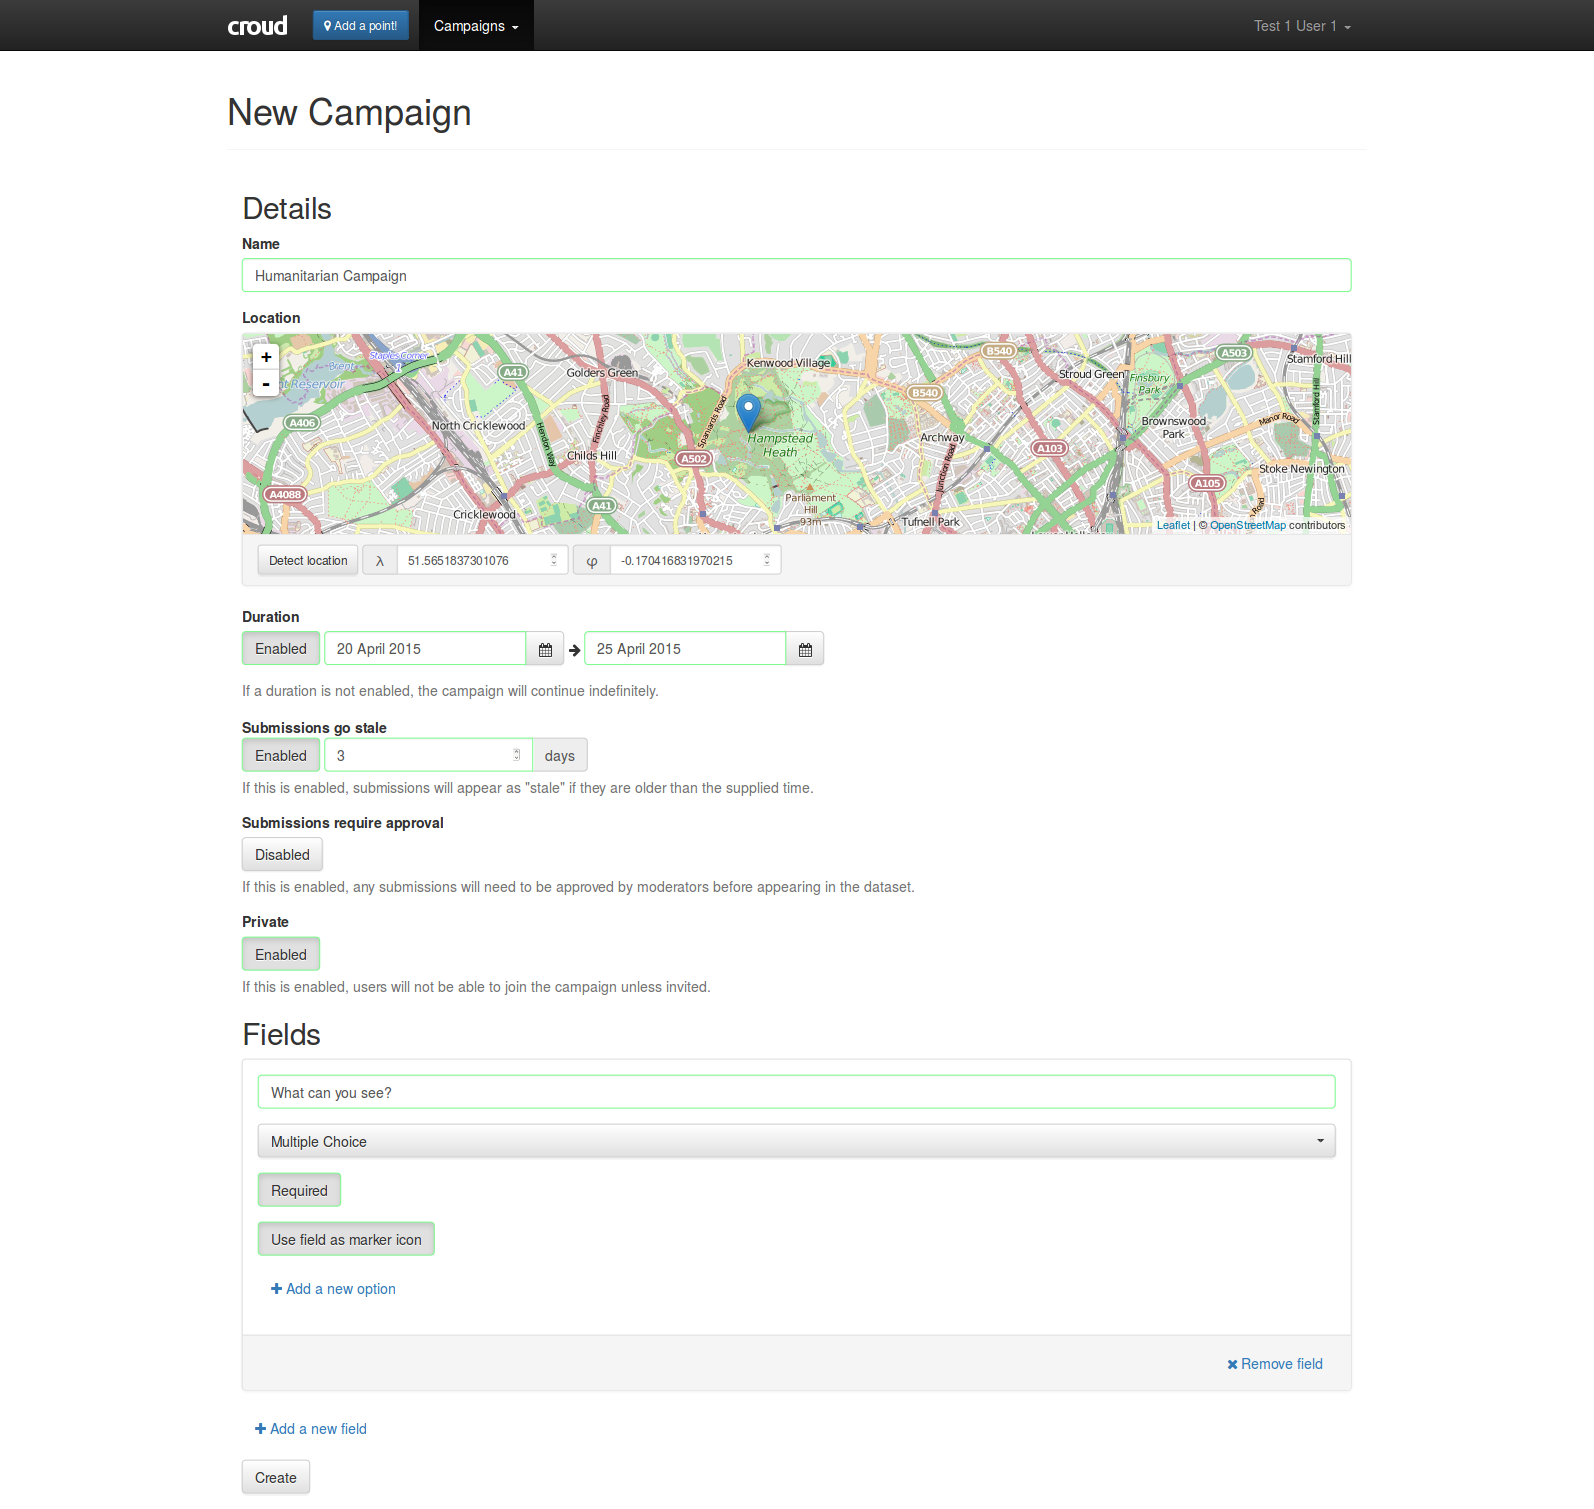
\includegraphics[width=4in]{eval-ca-3}}
			\caption{Campaign A form completed. Hampstead Heath is having a humanitarian crisis.}
			\label{fig:eval-ca-3}
		\end{figure}

		\begin{figure}[ht]
			\centering
			\fbox{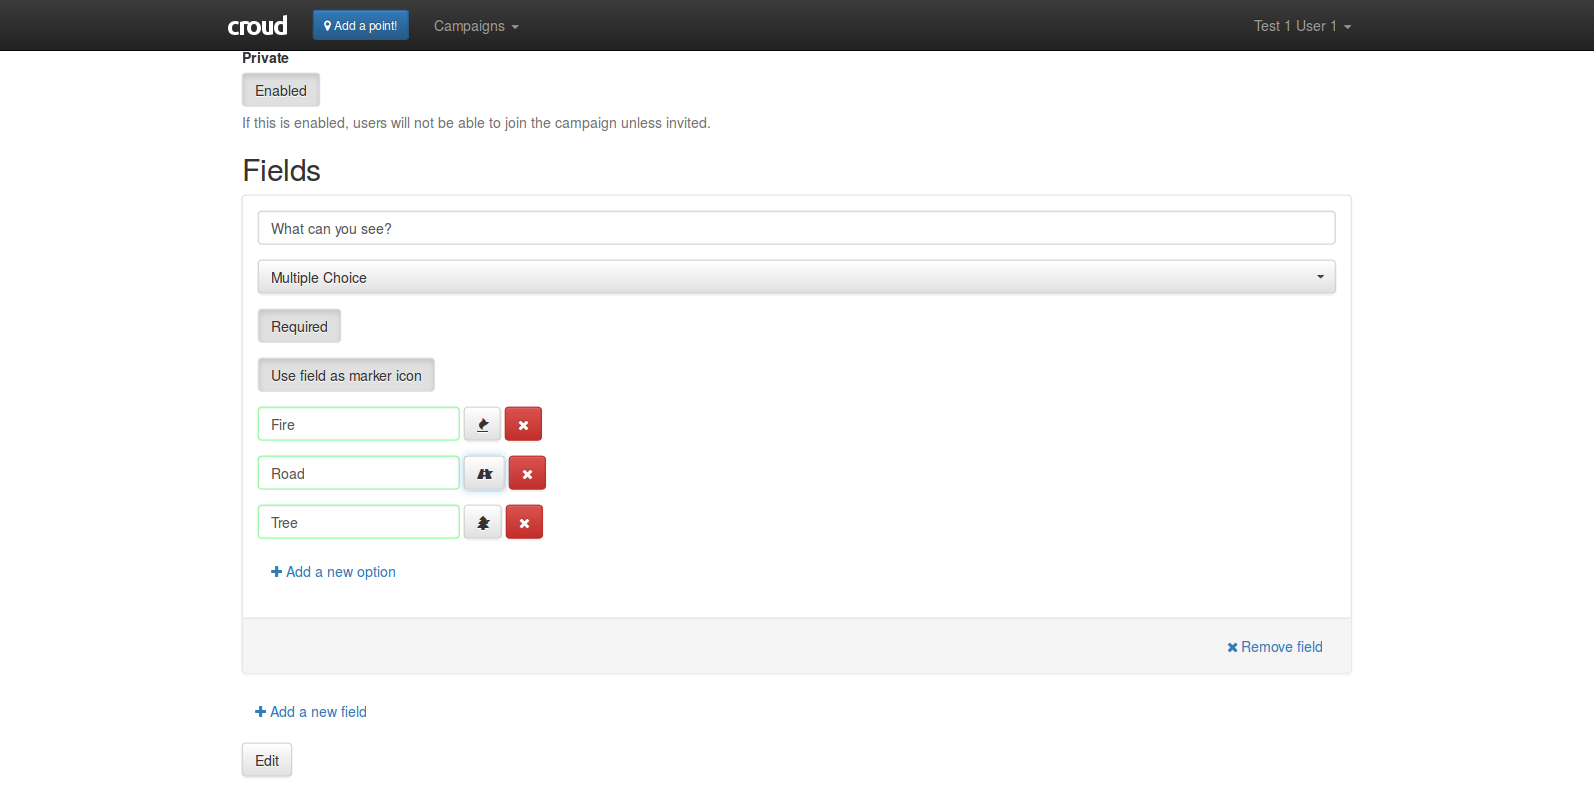
\includegraphics[width=4in]{eval-ca-5}}
			\caption{Configuration of options for multiple choice field.}
			\label{fig:eval-ca-5}
		\end{figure}


		\begin{figure}[ht]
			\centering
			\fbox{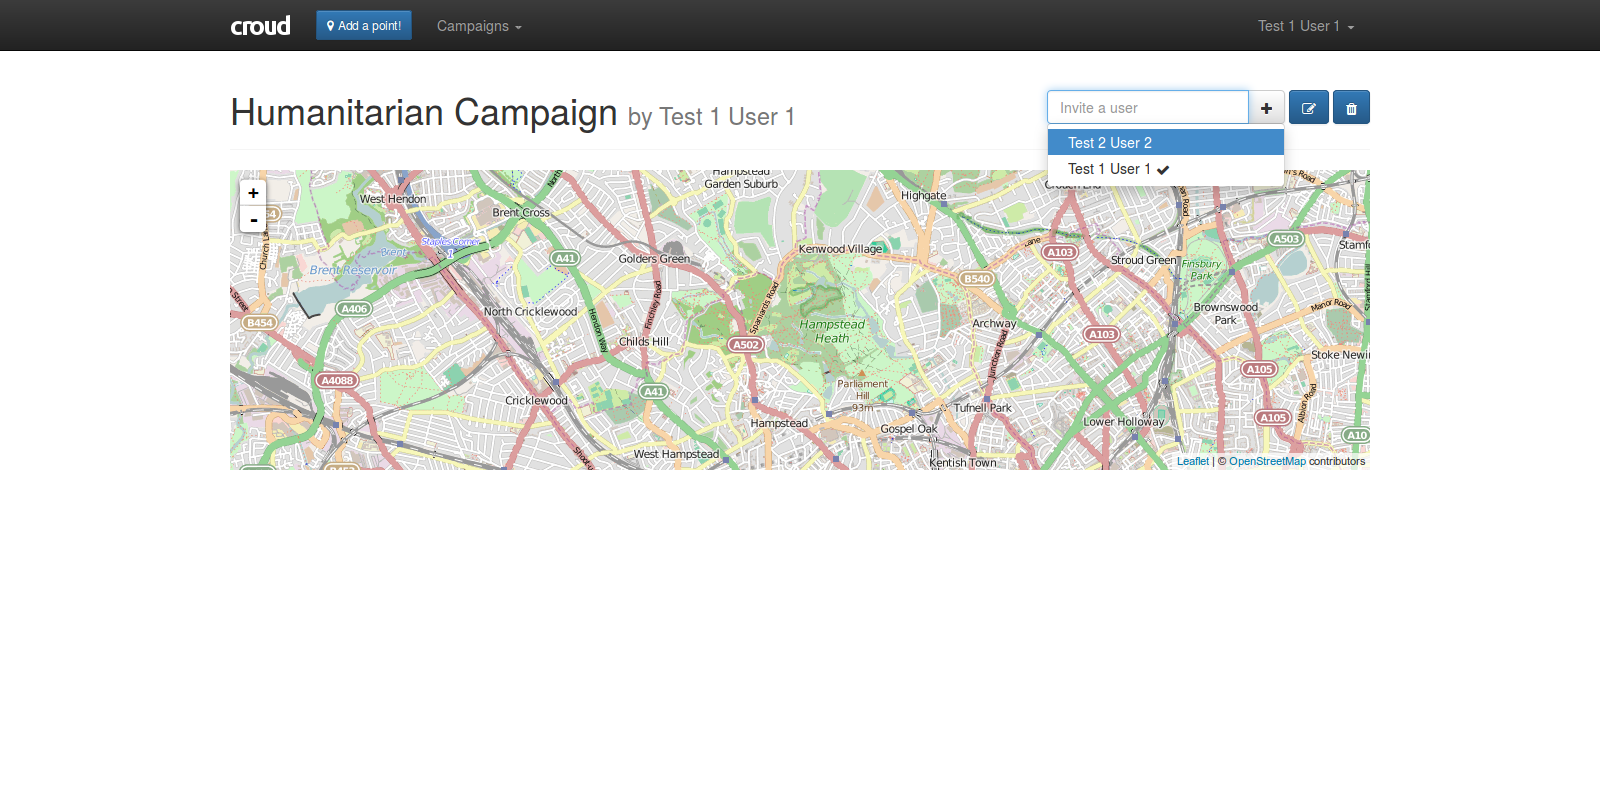
\includegraphics[width=4in]{eval-ca-6}}
			\caption{Adding \texttt{test2} to the private Campaign.}
			\label{fig:eval-ca-6}
		\end{figure}

		\begin{figure}[ht]
			\centering
			\fbox{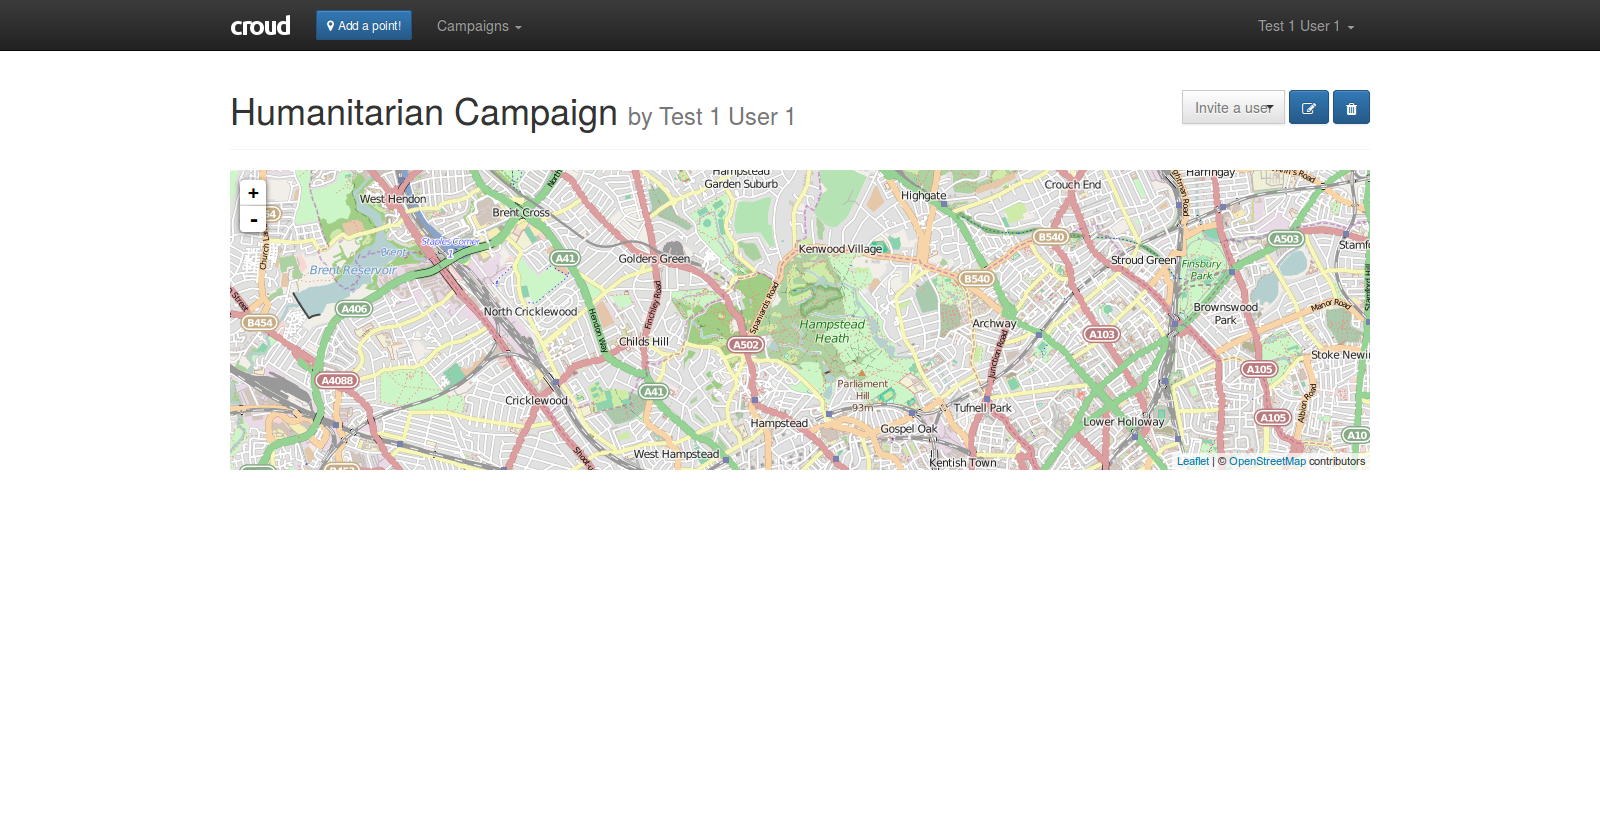
\includegraphics[width=4in]{eval-ca-4}}
			\caption{Campaign A ready to be used.}
			\label{fig:eval-ca-4}
		\end{figure}

		\FloatBarrier
		\subsection{Creating Campaign B}

		\begin{figure}[ht]
			\centering
			\fbox{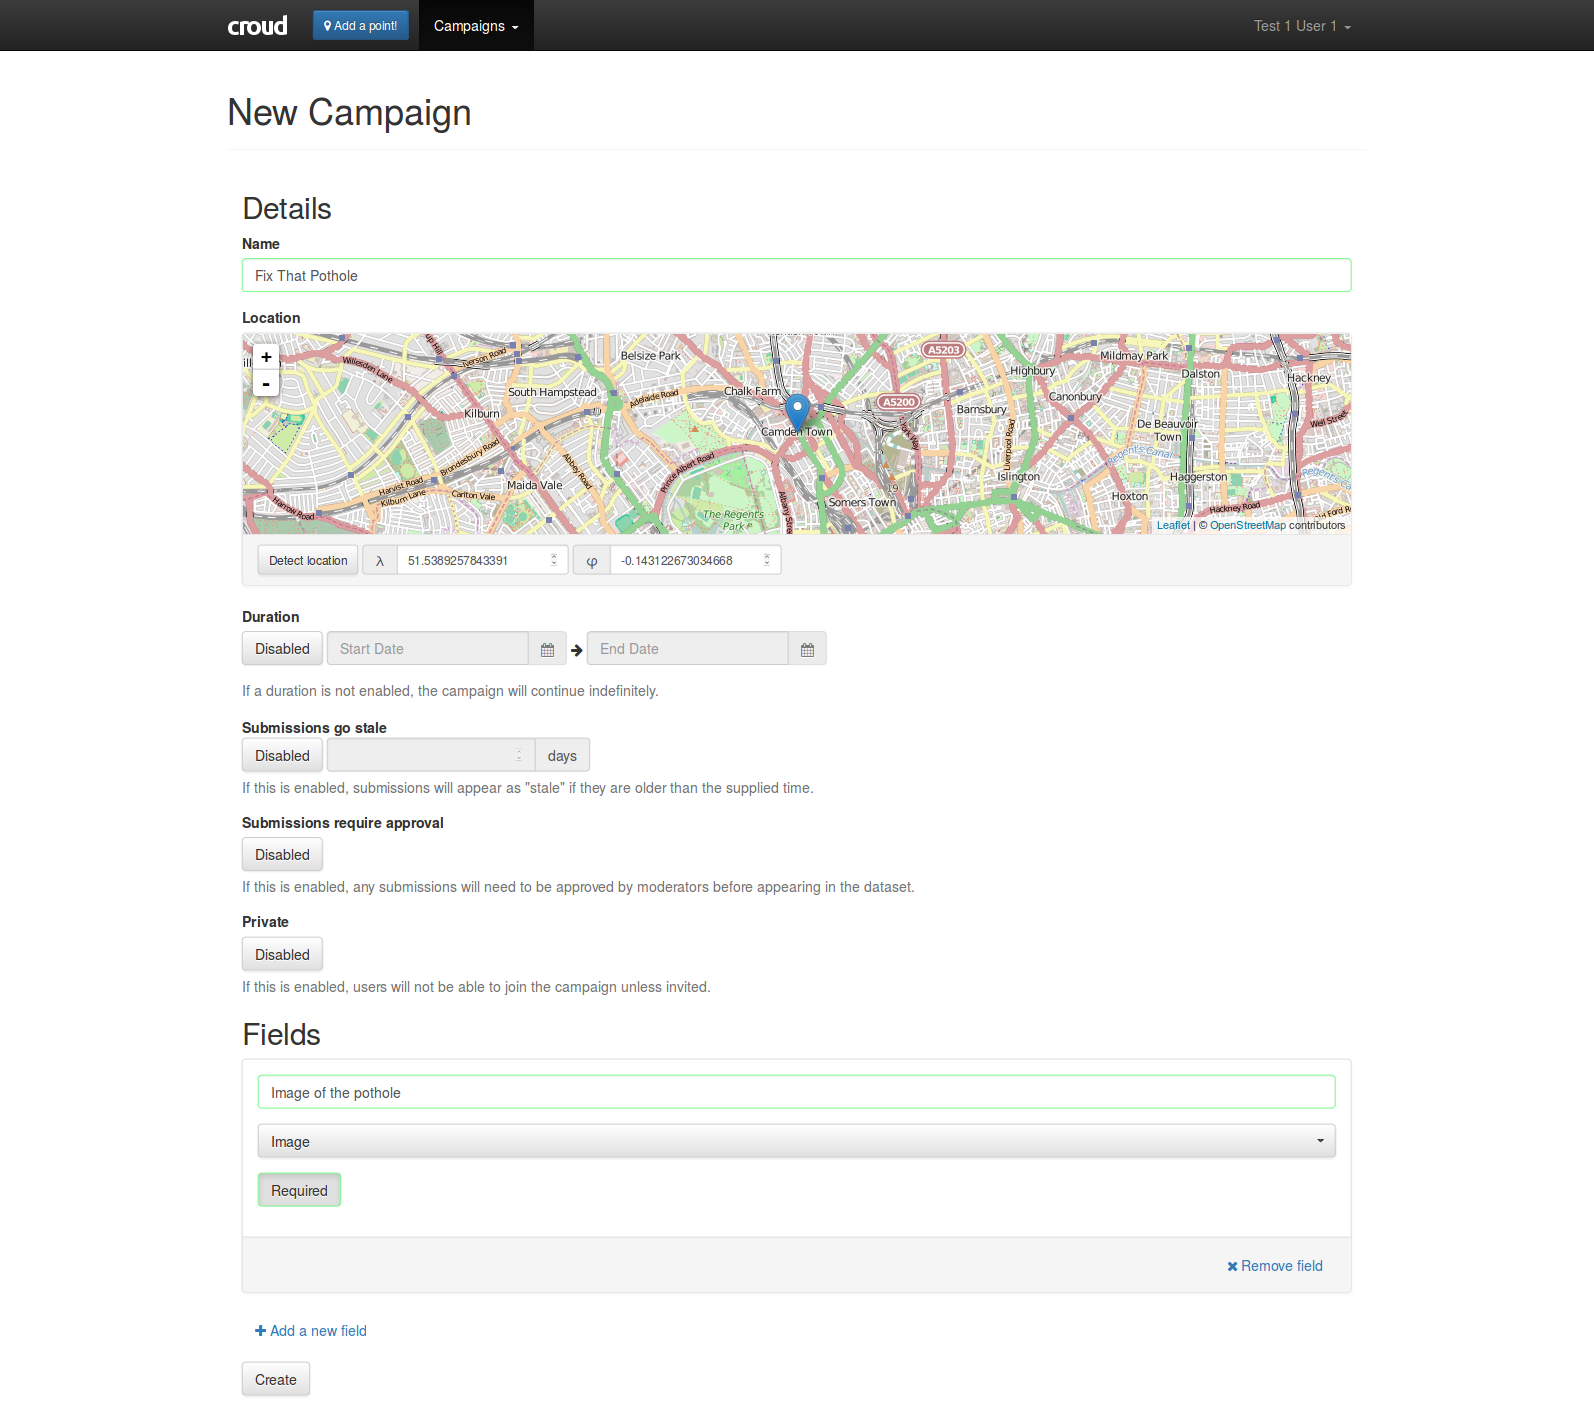
\includegraphics[width=4in]{eval-cb-1}}
			\caption{Campaign B form completed.}
			\label{fig:eval-cb-1}
		\end{figure}

		\FloatBarrier
		\subsection{Submitting Points to Campaign A}

		\begin{figure}[ht]
			\centering
			\fbox{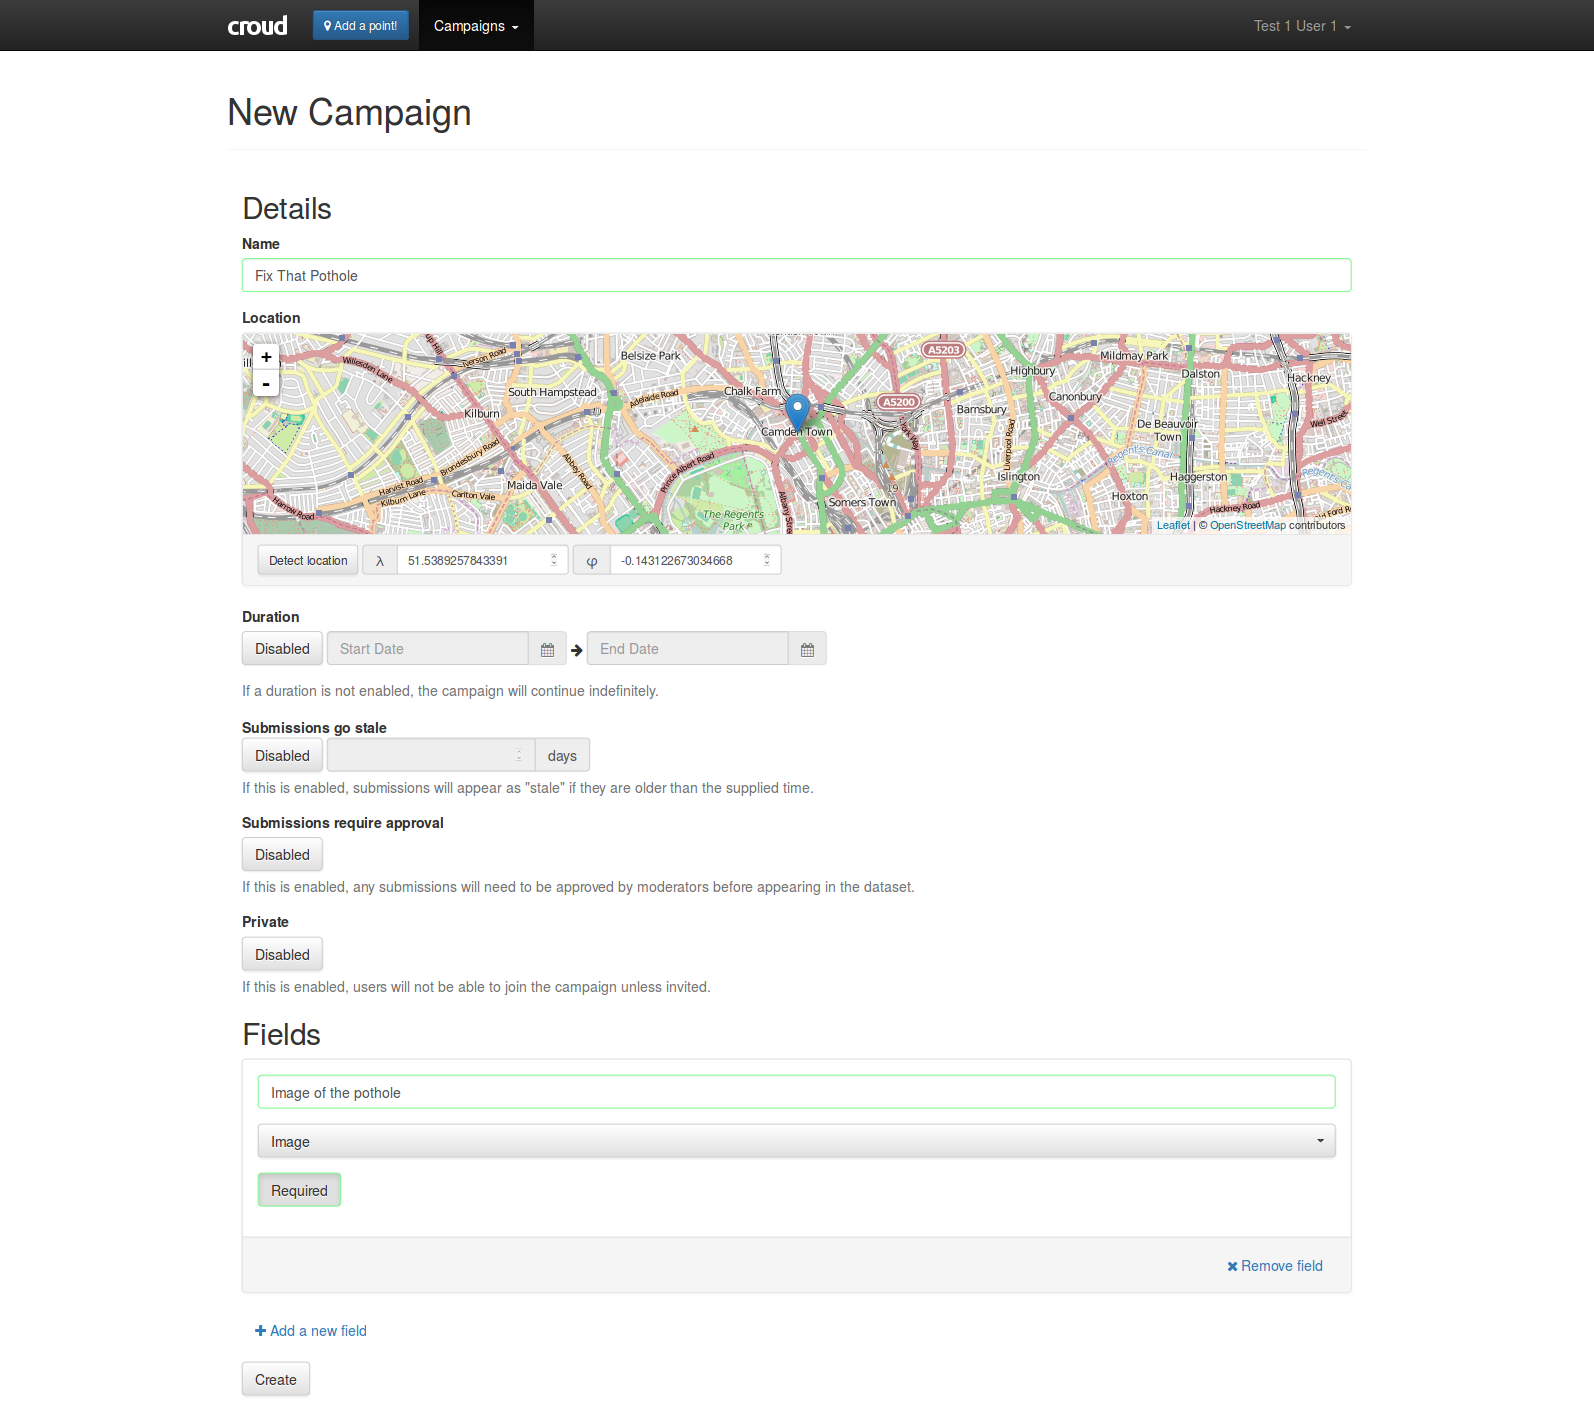
\includegraphics[width=4in]{eval-cb-1}}
			\caption{Selecting Campaign A (``Humanitarian Campaign'').}
			\label{fig:eval-submita-1}
		\end{figure}

		\begin{figure}[ht]
			\centering
			\fbox{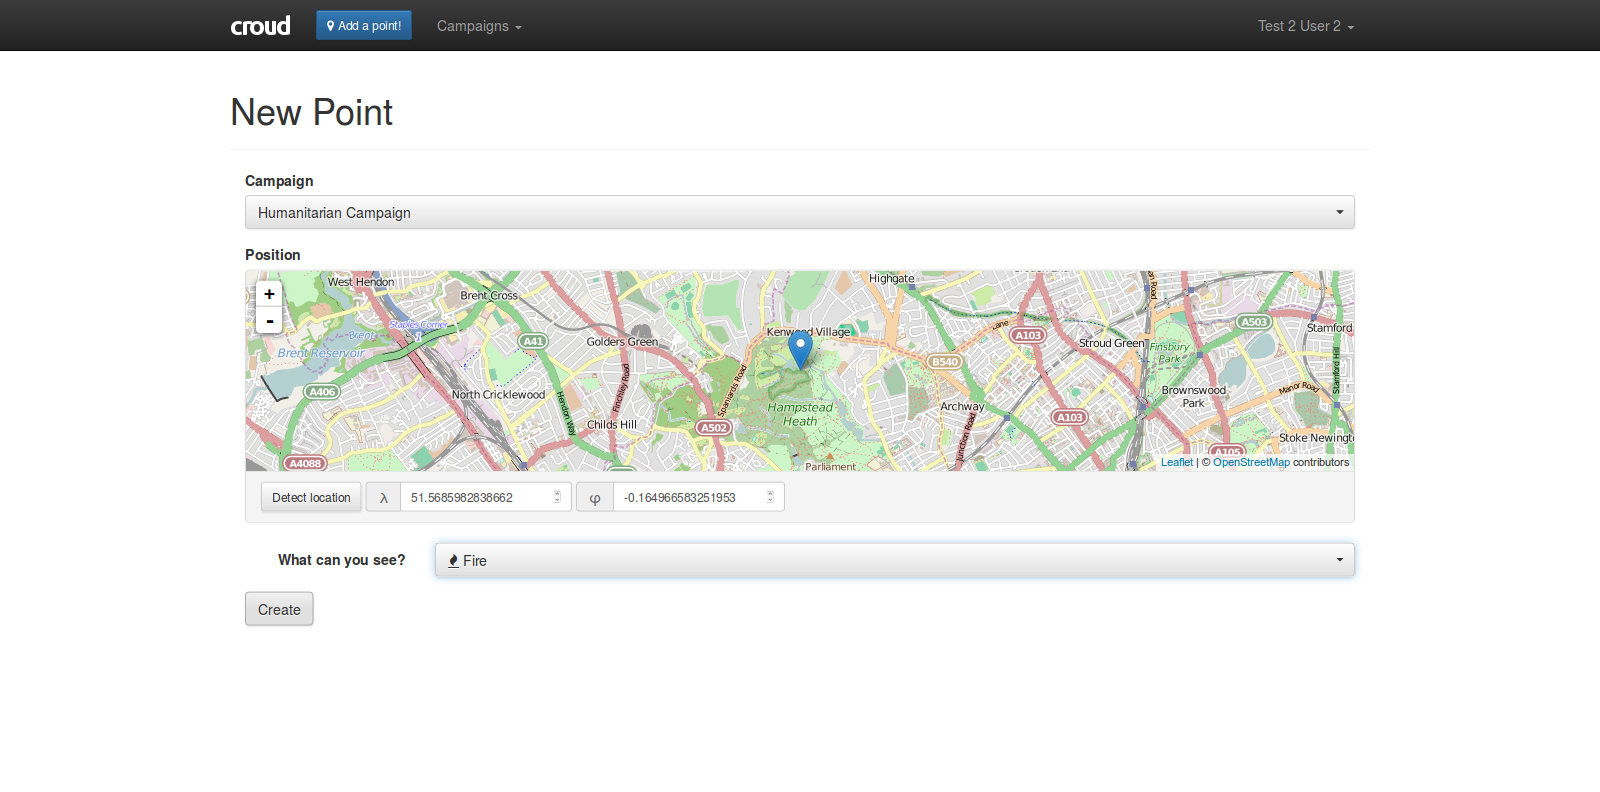
\includegraphics[width=4in]{eval-submita-2}}
			\caption{Filled in the Point information.}
			\label{fig:eval-submita-2}
		\end{figure}

		\begin{figure}[ht]
			\centering
			\fbox{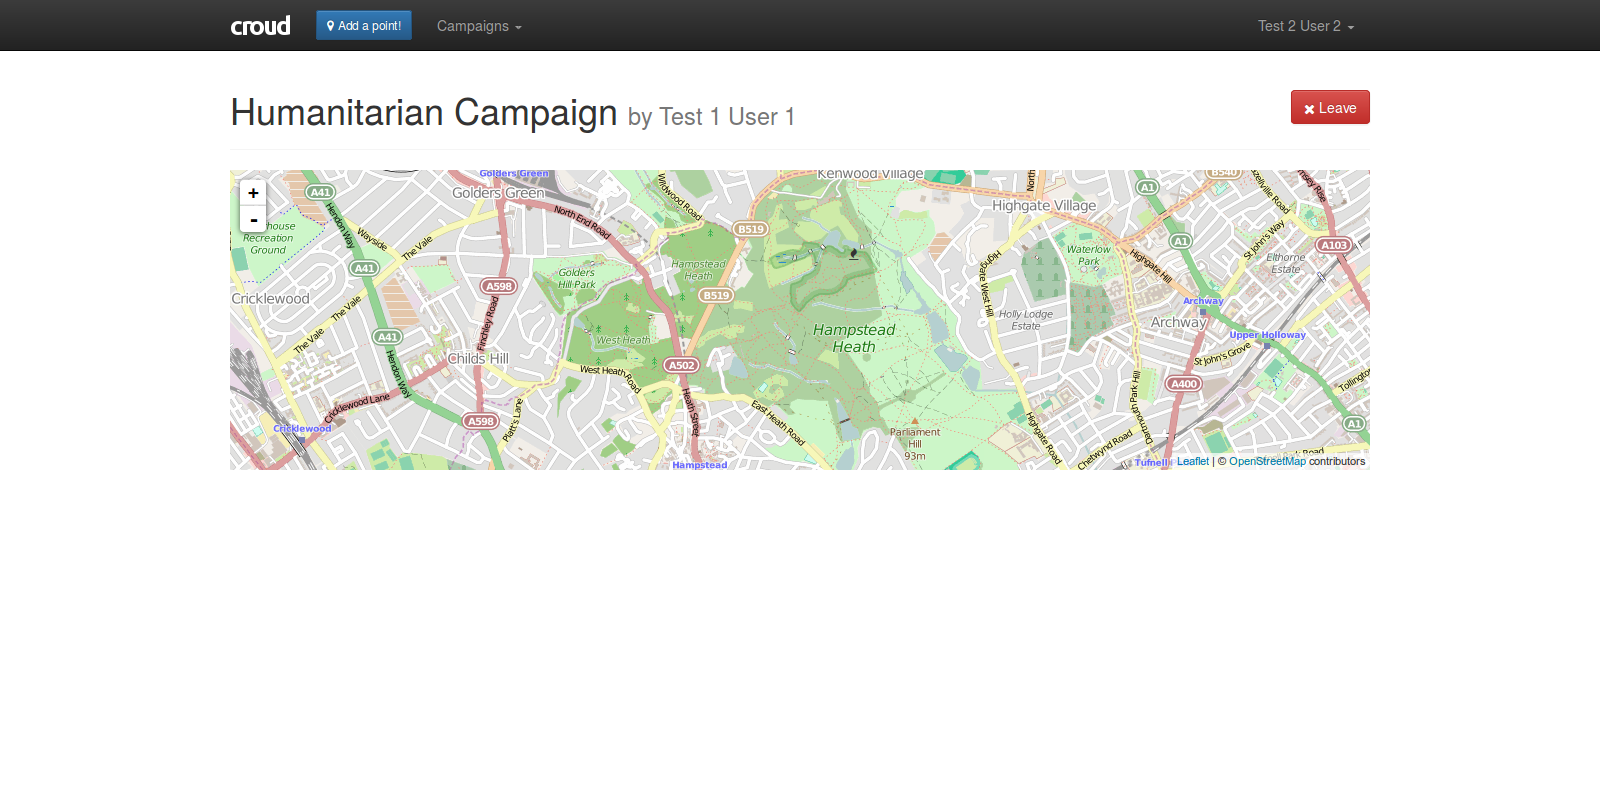
\includegraphics[width=4in]{eval-submita-3}}
			\caption{Campaign A now appears with a ``fire'' symbol where the point was placed.}
			\label{fig:eval-submita-3}
		\end{figure}

		\begin{figure}[ht]
			\centering
			\fbox{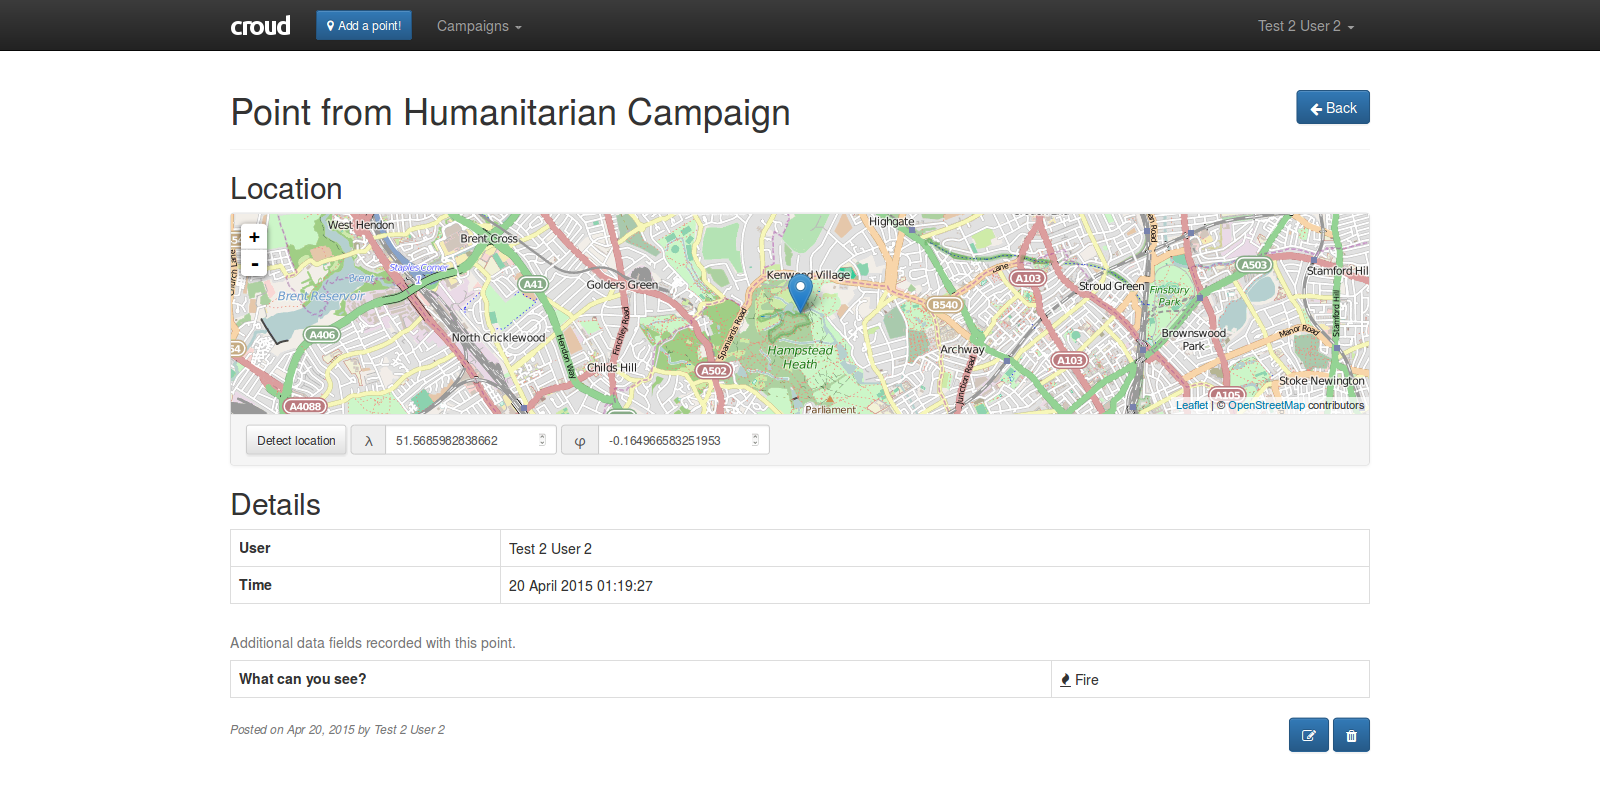
\includegraphics[width=4in]{eval-submita-4}}
			\caption{Clicking the ``fire'' symbol reveals this full information page for that Point.}
			\label{fig:eval-submita-4}
		\end{figure}

	\section{Conclusion}
	\label{sec:conclusion}

		Based on the evaluation in the previous section, it is clear that the framework can indeed be used to start a breadth of different crowdsourcing campaigns with the same interface. The campaigns were quick to create and were quick for users to upload data.

		Users with interest in data who would normally have little reach could use the platform to create Campaigns and build a base of interested contributors who might find the Campaign by reading browsing through the available projects.

		\subsection{Future changes}

		The framework currently exists as a proof of concept and there are a number of features that could be added to improve the system, attracting more users and widening the application of the framework.

		\begin{itemize}
			\pitem{More customisation of Campaigns} Campaigns could have descriptions, cover images, Twitter feeds and other additions to make them feel more social. At the moment the framework displays the name of the Campaign and the map data, but this could easily be built into a profile page for each Campaign.
			\pitem{Organisations} Rather than Campaigns being owned by Users, they could instead be part of Organisations. This would allow Campaigns by a single Organisation to be shown together, like \emph{American Red Cross} for example. Users could be given roles in Organisations that would allow them to create Campaigns, or cause them to automatically become moderators of any new Campaigns in that Organisation.
			\pitem{More field types} Although the five that currently exist fit the requirements of the existing projects this framework is intended to replace, there are many other field types that could be added with more time to build the software. For example: star rating scale, audio upload, or barcode for the mobile application.
			\pitem{Social aspect} At the moment Users are quite opaque to each other, with little by way of ``public profile''. In the future, the application could be expanded to include optional sharing of activity for Users, so that Users can find new Campaigns to contribute to by looking at what their friends are doing.
			\pitem{Suggested Campaigns} As mentioned earlier in the document, using suggestion algorithms and given a big enough user base it would be possible to suggest Campaigns for a User to contribute to based on the Campaigns they already have joined.
			\pitem{Stale Point reminders} When a Point becomes stale, a user could be reminded via email to check that submission again, or other Users who have submitted data nearby could be prompted to check out that location.
			\pitem{Motivational strategies} The utility of the framework would be greatly improved by the availability of common motivational strategies in the framework. For example: being able to configure some points system for Users submitting data; or providing some method of micropayments to Users for each Point they submit.
			\pitem{More relevant icon set for multiple choice field} At the moment the framework uses \emph{FontAwesome} because it has a large set of icons and is already loaded on the site for iconographic use. However, when projects like \emph{Maki} by \emph{Mapbox} for ``point of interest icon sets'' get bigger and include more icons, the system could easily be switched to use them.
		\end{itemize}

	\bibliographystyle{Croud}
	\bibliography{Croud}

	\clearpage
	\begin{appendices}
	\oldsection{API Documentation}
	\label{sec:api-docs}
	\end{appendices}

\end{document}
